%\documentclass[b5paper,final,11pt,fleqn,twoside]{book}

\documentclass[a4paper,twoside,12pt]{report}
\usepackage{times}
\usepackage{graphics}

\usepackage{weso}

%
% cabeceras.tex
%
% Copyright 2003, Diego Berrueta Muñoz
%
% Cabeceras comunes
%

\usepackage[T1]{fontenc}

%Glosario

\usepackage[toc,style=treenoname,order=word,counter=section]{glossaries}

\usepackage{xspace}


\usepackage{tikz,times}
\usetikzlibrary{mindmap,backgrounds}

% cambia algunas fuentes (utilidad dudosa)
\usepackage[scaled=0.92]{helvet}
\usepackage{pifont}
\usepackage{courier}

% cambia algunas fuentes en modo matemático a Palatino
\usepackage{mathpazo}

% españolización
\usepackage[spanish]{babel}
\usepackage[utf8]{inputenc}
%\extrasspanish

% gráficos y colores
\usepackage{rotating}
\usepackage{graphicx}
\usepackage{color}
%\usepackage[all]{xy}
%\usepackage{pstricks}
\usepackage{pst-node}
%\usepackage[dvips,usenames]{pstcol}
%\usepackage{pdftricks}
%\usepackage{pst-uml}  % para hacer diagramas UML
%\usepackage{rail}     % para hacer diagramas de gramáticas

% mejoras visuales
\usepackage{enumerate}
\usepackage{fancyhdr}  % para configurar los encabezados
\usepackage{fancybox}  % para hacer cajitas
\usepackage[normal,oneline,sf,bf]{caption2}
\usepackage{titlesec}  % para configurar los títulos de sección
\usepackage{paralist}


\usepackage{epigraph}

% citas, referencias e índices
\usepackage{cite}
%\usepackage{citesort}   % da errores al compilar
\usepackage{makeidx}

% incrustaciones de código fuente
%\usepackage[norules,nolineno]{lgrind}
\usepackage{verbatim}
\usepackage{listings}
%\usepackage{noweb,a4wide}


%\usepackage{textcomp}
\usepackage[right]{eurosym}

% columnas
\usepackage{multicol}

% tablas
\usepackage{longtable}
%\usepackage{ltxtable}

% impresión elegante de URLs
\usepackage{url}

\makeatletter
\def\url@pfcstyle{%
  \@ifundefined{selectfont}{\def\UrlFont{\sf}}{\def\UrlFont{\small\ttfamily}}}
\makeatother
%% Now actually use the newly defined style.
\urlstyle{pfc}


% márgenes
\usepackage[a4paper, left=30mm, right=20mm, top=25mm, bottom=25mm]{geometry}
%\usepackage[a4paper, left=20mm, right=20mm, top=25mm, bottom=25mm]{geometry}

% 
% \usepackage[a4,center,cam]{crop}
\usepackage{blindtext}

% salida en PDF navegable
%\usepackage{hyperref}
\usepackage[plainpages=false,colorlinks, linkcolor=black]{hyperref}

% quitar en versión final
%\usepackage{showkeys}   % depuración de etiquetas y referencias
%\usepackage{showidx}    % depuración de índice

% configuración del paquete "listings"

\lstset{%
        %language=Java,
	basicstyle=\footnotesize\sffamily,
	keywordstyle=\bfseries, %\color{darkred}
 	stringstyle=\itshape, %\color{violet}
 	commentstyle=\itshape, %\color{blue}
 	showspaces=false,
 	showtabs=false,
 	showstringspaces=false,
 	frame=trBL,
        frameround=tttt,
        %backgroundcolor=\color{lightyellow},
	inputencoding=utf8,
 	extendedchars=true,
 	numbers=none,
        aboveskip=0.5cm,
        belowskip=0.5cm,
        xleftmargin=1cm,
        xrightmargin=1cm,
	breaklines=true
}
\definecolor{darkred}{rgb}{0.5, 0, 0}
\definecolor{violet}{rgb}{1, 0, 1}
\definecolor{lightyellow}{rgb}{1,1,0.8}


%%%%%%%%%%%%%%%%%%%%%%%%%%%%%%%%%%%%%%%%%%%%%%%%%%%%%%%%%%%%%%%%%%%%%%
% cabeceras y pies de página (con el paquete "fancyhdr")
\headheight 15pt
%\addtolength{\headwidth}{\marginparsep}
%\addtolength{\headwidth}{\marginparwidth}
%\renewcommand{\chaptermark}[1]{\markboth{\MakeUppercase{#1}}{}}
%\renewcommand{\sectionmark}[1]{\markright{\thesection\ #1}}
%\fancyhead[LE,RO]{\textbf{\thepage}}
%\fancyhead[RE]{\textit{\leftmark}}
%\fancyhead[LO]{\rightmark}
%\fancyfoot[LCR]{}
\fancyhead{} % Todos los campos en blanco en la cabecera
\fancyfoot{} % Lo mismo al pie
\fancyhead[RO, LE]{\thepage}
\fancyhead[LO, RE]{\slshape\leftmark}
\renewcommand{\headrulewidth}{0.5pt}
\renewcommand{\footrulewidth}{0.5pt}


%%%%%%%%%%%%%%%%%%%%%%%%%%%%%%%%%%%%%%%%%%%%%%%%%%%%%%%%%%%%%%%%%%%%%%
% títulos de secciones (con el paquete "titlesec")
\titleformat{\chapter}[display]
	{\fontfamily{pag}\selectfont\Huge}
	{\LARGE\chaptertitlename\ \thechapter}{20pt}{\bfseries}
\titleformat{\section}
	{\fontfamily{phv}\selectfont\LARGE}
	{\thesection}{1em}{\bfseries}[\titlerule]
\titleformat{\subsection}
	{\fontfamily{phv}\selectfont\Large}
	{\thesubsection}{1em}{\bfseries}
\titleformat{\subsubsection}
	{\fontfamily{phv}\selectfont\large}
	{\thesubsubsection}{1em}{\bfseries}


%%%%%%%%%%%%%%%%%%%%%%%%%%%%%%%%%%%%%%%%%%%%%%%%%%%%%%%%%%%%%%%%%%%%%%
% espaciado entre párrafos
\addtolength{\parskip}{+0.2cm}


%%%%%%%%%%%%%%%%%%%%%%%%%%%%%%%%%%%%%%%%%%%%%%%%%%%%%%%%%%%%%%%%%%%%%%
% salida en PDF navegable (con el paquete "hyperref")
\hypersetup{bookmarks,
	bookmarksnumbered,
%	colorlinks, % quitar en las versiones impresas
	hyperindex,
	%linkcolor=red,
	%anchorcolor=black,
	%citecolor=green,
	citecolor=violet,
	%filecolor=magenta,
	%menucolor=red,
	%pagecolor=red,
	%urlcolor=cyan,
	pdftitle={PhD. Dissertation-Jose María Alvarez Rodríguez},
	pdfauthor={Jose María Alvarez Rodríguez}
	pdffitwindow,
	plainpages=false,
	pageanchor=false,
	pdfstartview={}}


%%%%%%%%%%%%%%%%%%%%%%%%%%%%%%%%%%%%%%%%%%%%%%%%%%%%%%%%%%%%%%%%%%%%%%
% profundidad de secciones y numeración
%\setcounter{tocdepth}{4}
\setcounter{secnumdepth}{3}


%%%%%%%%%%%%%%%%%%%%%%%%%%%%%%%%%%%%%%%%%%%%%%%%%%%%%%%%%%%%%%%%%%%%%%
% división silábica
\hyphenation{pu-bli-ca-ción con-tex-tua-li-za-ción pro-ble-mas Mi-nis-te-rio li-ci-ta-ción si-guien-tes desa-rro-llar con-tra-ta-ción pan-europea fa-ci-li-tar in-ter-opera-bility
 elec-tró-ni-ca li-ci-ta-do-ras he-te-ro-gé-neos res-trin-gi-do cons-cien-te de-sa-rro-lla-da mo-de-lo paí-ses ge-ne-ra-da
 par-ti-ci-pa-ción ad-mi-nis-tra-ti-vos bi-blio-gra-fía re-gis-tra-do-ra ad-mi-nis-tra-ti-va ca-rac-te-rís-ti-cas
 Pa-ra-le-la-men-te des-cri-ben vo-ca-bu-la-rio me-dian-te do-cu-men-to di-fe-ren-tes bi-blio-gra-fía mo-de-lo
 ve-ri-fi-ca rea-li-zar res-tric-ciones Por ejem-plo su-ge-ren-cias mo-de-los rea-li-za si-guien-do he-te-ro-gé-neas ello
 ra-zo-na-ble li-mi-ta-cio-nes reu-ti-li-cen ini-cia-ti-va va-ria-da exis-ten ob-te-ner con-ti-nua-men-te me-dian-te ins-ti-tu-ción
 pro-pues-ta pu-bli-ca-ción ca-tá-lo-go mo-ni-to-ri-za-ción vi-sua-li-za-ción mo-de-los co-rres-pon-dien-tes
 re-fe-ren-cia re-la-ti-vas par-ti-cu-lar  ele-men-to mo-de-la-do se-le-ccio-na-do pro-du-cción Re-con-ci-lia-ción des-crip-cio-nes broader-Transitive 
 de-pen-dien-do Ca-tá-lo-gos vo-ca-bu-la-rios Pro-pie-ta-rio des-plie-gue De-sa-rro-lla-dor mo-de-lar res-pues-ta si-mi-la-res rea-li-za-do SE-RI-MI 
Evol-ving ha-bi-li-tar rea-li-za-ción pu-bli-ca-ción ge-ne-ra-ción rea-li-za-ban ac-tua-li-za-ción ac-ce-so ha-cer es-tán-dar 
vo-ca-bu-la-ry con-si-de-ra-do des-cri-bir pu-bli-car pu-bli-ca-dos ta-xo-nó-mi-ca Pro-duct-on-to-lo-gy Va-lo-res in-terope-ra-bi-li-dad MOL-DEAS 
man-te-ni-mien-to re-pre-sen-tar ta-xo-no-mías des-crip-ción ge-ne-ra cons-truc-ción re-pre-sen-tan-do rea-li-za-das trans-fe-ren-cia 
uti-li-za-ble pu-bli-ca be-ne-fi-cios res-pon-sa-bi-li-da-des rea-li-zan Ad-mi-nis-tra-ción con-ti-nua-ción prio-ri-ta-rio ICT 
in-terope-ra-ble ge-ne-ra-do con-fi-gu-ra-cio-nes rea-li-zan-do rea-lis-ta má-xi-mo Cons-ti-tu-yen-do pro-ble-ma po-si-bi-li-dad ma-yor coo-pe-ra-ción 
ra-zo-na-mien-to Des-crip-tion con-cep-tua-li-za-ción de-sa-rro-lla-dos ope-ra-do-res axio-mas go-bier-no or-ga-nis-mos éxi-to 
si-guien-te do-mi-nios pro-duc-ción Na-tio-nal orien-ta-da ló-gi-ca in-di-vi-duos di-se-ña-do for-ma-li-za-dos ta-xo-no-mía 
auto-má-ti-ca ca-li-dad re-co-men-da-ble ad-mi-nis-tra-ti-vo su-mi-nis-tre error ca-rac-te-rís-ti-ca ele-men-tos he-rra-mien-tas 
eva-lua-ción res-pec-to Ad-mi-nis-tra-cio-nes ex-pe-ri-men-tal orien-ta-das re-gis-tros do-cu-men-tos má-xi-ma je-rar-quía 
sa-tis-fac-to-rios obs-tan-te con-su-mi-dos con-fe-ren-cias SPARQL rea-li-za-dos va-lo-ran eco-no-mi-zar fle-xi-ble ex-pe-dien-te 
pro-ce-di-mien-to usan-do ame-ri-ca-nas fa-mi-lia ni-vel ra-zo-na-do-res re-pre-sen-ta-ción lo-ca-li-za-do Man-ches-ter 
en-ri-que-ci-mien-to he-rra-mien-ta rea-li-zar-se prio-ri-ta-rios Li-ci-ta-cio-nes ne-ce-sa-rios ma-te-ria-li-zan es-pe-cia-li-zán-do-se 
Com-pu-ting pla-ni-fi-ca-ción cua-li-ta-ti-va de-sa-for-tu-na-da-men-te li-de-ra-do ma-te-ria-li-za-do Cons-tructs 
ma-te-ria-li-za WESO en-ten-di-mien-to MOLDEAS ela-bo-ra-ción re-fe-ren-te re-gis-tra-tion uni-la-te-ral po-si-bi-li-tar ope-rar 
in-ter-ope-ra-bles ad-mi-nis-tra-ti-vas fle-xi-bi-li-dad auto-no-mía co-mer-cio procesa-miento de-sa-rro-llan-do meta-in-for-ma-ción 
apro-pia-dos li-mi-ta-do es-pe-cia-li-za-ción ló-gi-cas in-de-pen-dien-te-men-te ge-ne-ral dis-po-ner dis-mi-nu-yen-do co-rrien-te 
rea-pro-ve-char de-sa-rro-llo ge-ne-ral Ins-ti-tu-te com-pu-ting pos-te-rior con-su-mi-da mi-llo-nes Fi-gu-ras cons-tan-te equi-va-len-cia ope-ra-cio-nes 
fac-to-ri-za-ción Res-pon-sa-bles Geo-Linked-Data reu-ti-li-za-ción co-rrec-tos trans-for-ma-ción bien con-si-guien-te des-cu-brien-do 
geo-rre-fe-ren-cia-ción pro-li-fe-ra-ción cum-pli-mien-to Ne-go-tia-ted uti-li-dad ma-nual es-pe-cia-li-za-ción ma-yo-ría mo-de-la 
des-cu-bri-mien-to rea-li-za-da pu-bli-can se-lec-cio-nar me-ca-nis-mos fun-cio-na-li-dad ve-ri-fi-car ines-pe-ra-dos re-gis-tro 
pro-pues-tos trans-pa-ren-te va-ria-bles bi-blio-te-ca bi-blio-te-cas adap-ta-bi-li-dad in-ter-co-ne-xión va-ria-ble vi-sua-li-zar 
ope-ra-ti-vo ge-ne-rar su-mi-nis-tra-dos va-li-da-ción su-mi-nis-tra-dores pro-pie-da-des hi-po-ni-mia re-cu-pe-ra-dos in-de-pen-dien-te-ment-te 
triun-fo reu-ti-li-za-ción ge-ne-ral apro-xi-ma-ción va-ria-bi-li-dad teó-ri-cas con-ti-nuo di-se-ño des-afor-tu-na-da-men-te In-dus-trial prin-ci-pios 
di-fe-ren-cia-das eva-lua-dos re-qui-si-tos co-la-bo-ra-cio-nes co-la-bo-ra-ción in-dus-tria-les Se-venth pon-de-ra-do re-po-si-to-rios 
ex-pe-ri-men-ta-les pu-bli-ci-tar co-la-bo-ra-ción bi-llo-nes Doc-to-ra-do re-so-lu-ción cul-tu-ra-les trans-cur-so Pa-rro-quias Lo-gics co-rrec-to 
sig-ni-fi-ca-do Aña-dien-do ope-ra-ción ma-ne-ra agi-li-zar con-fian-za per-so-na-les in-al-te-ra-dos re-la-ti-vos des-cri-bien-do 
se-ña-la-das vo-ca-bu-la-ries con-tex-tua-li-za-da Ba-rras cir-cuns-cri-bién-do-se for-ma-li-za-ción fa-ci-li-tan-do re-ali-men-ta-ción 
re-fe-ren-cias ma-ni-fes-tar-se CKAN lo-ca-li-dad dia-gra-ma ver-da-de-ra-men-te es-ta-ble-ci-mien-to con-si-de-ra ta-reas co-rrec-ta 
co-he-ren-te pos-te-rior-men-te apro-pia-das exac-tos va-rios pro-pues-to ex-pe-ri-men-to re-fe-ren-tes orien-ta-dos ha-bi-tual con-cre-tas 
con-fi-gu-ran afi-lia-ción Gi-ner va-lo-ra-ción res-pon-sa-bi-li-dad}   

%%Tablas
\addto\captionsspanish{
        \def\listtablename{\'Indice de tablas}%
        \def\tablename{Tabla}} 

%%%Math
\usepackage{latexsym}
\usepackage{amsmath}
\usepackage{amssymb}
\usepackage{amsthm}

\usepackage{algorithm}
\usepackage{algorithmic}
\usepackage{multirow}
\usepackage{rotating}


\newtheorem{theorem}{Theorem}[section]
\newtheorem{proposition}[theorem]{Proposición}
\newtheorem{lemma}[theorem]{Lema}
\newtheorem{definition}[theorem]{Definición}
\newtheorem{examples}[theorem]{Ejemplos}
\newtheorem{remarks}[theorem]{Remarks}
\newtheorem{corollary}[theorem]{Corolario}
\newtheorem{remark}[theorem]{Remark}
\newtheorem{example}[theorem]{Ejemplo}
\newtheorem{conjecture}[theorem]{Conjecture}
\newtheorem{note}[theorem]{Nota}



\newsavebox\FrameBox
\newenvironment{Frame}{%
  \par\setbox\FrameBox\hbox\bgroup\minipage{0.9\textwidth}\parskip\baselineskip\ignorespaces
}{%
  \endminipage\egroup\fbox{\box\FrameBox}\par
}

\newcommand{\si}{$\oplus$\xspace}
\newcommand{\no}{$\ominus$\xspace}
\newcommand{\na}{$\odot$\xspace}


%Extraer
\newcommand{\linkeddata}{\textit{Linked Data}\xspace}
\newcommand{\opendata}{\textit{Open Data}\xspace}
\newcommand{\lod}{\textit{Linking Open Data}\xspace}
\newcommand{\ogd}{\textit{Open Government Data}\xspace}
\newcommand{\datasets}{\textit{datasets}\xspace}
\newcommand{\dataset}{\textit{dataset}\xspace}
\newcommand{\provenance}{\textit{provenance}\xspace}
\newcommand{\trust}{\textit{trust}\xspace}
\newcommand{\egov}{\textit{e-government}\xspace}
\newcommand{\pusi}{\textit{Public Sector Information}\xspace}
\newcommand{\gd}{\textit{Government Data}\xspace}
\newcommand{\wod}{Web de Datos\xspace}
\newcommand{\wode}{\textit{Web of Data}\xspace}
\newcommand{\eproc}{\textit{\gls{e-Procurement}}\xspace}
\newcommand{\gld}{\textit{Government Linked Data}\xspace}


%
% utilidades.tex
%
% Copyright 2003, Diego Berrueta Muñoz
%
% Algunos comandos y entornos utilizados
%


%%%%%%%%%%%%%%%%%%%%%%%%%%%%%%%%%%%%%%%%%%%%%%%%%%%%%%%%%%%%%%%%%%%%%%
% Para llamadas de atención al margen

\reversemarginpar

\newcommand{\attention}{%
  \mbox{}\marginpar{\raggedleft \large\bfseries ! $\rightarrow$}%
}

\newcommand{\InlineFIXME}[1]{%
  {\bfseries\color{red} FIXME: #1}%
}

\newcommand{\FIXME}[1]{%
  \attention{}{\color{red}\bfseries #1}%
}


%%%%%%%%%%%%%%%%%%%%%%%%%%%%%%%%%%%%%%%%%%%%%%%%%%%%%%%%%%%%%%%%%%%%%%
% Comandos específicos de este proyecto

\newcommand{\FechaEntregaPFC}{Octubre 2007}
\newcommand{\TituloPFC}{Activación de conceptos en ontologías mediante el algoritmo de \textit{Spreading Activation}}
\newcommand{\NumeroPFC}{1072029}
\newcommand{\AreaPFC}{LENGUAJES Y SISTEMAS INFORMÁTICOS}
\newcommand{\AutorPFC}{Jose María Álvarez Rodríguez}
\newcommand{\TutorPFC}{José Emilio Labra Gayo}

\newcommand{\Curry}{Curry}
\newcommand{\Zinc}{Zinc}
\newcommand{\Prelude}{Prelude}

\newcommand{\toriginal}[1]{\textit{#1}}

\newcommand{\simbolo}[1]{ %
  \textbf{\texttt{#1}} %
}




\input{../portada}


\input{../bibliografia-utils}


\makeindex

\makeglossaries
\loadglsentries{glosario}


%%%%%%%%%%%%%%%%%%%%%%%%%%%%%%%%%%%%%%%%%%%%%%%%%%%%%%%%%%%%%%%%%%%%%%
\begin{document}


\title{A/EN01-00-Informe \textit{Open Data}}


\author{
{Jose María Alvarez-Rodríguez (WESO)\\
josem.alvarez@weso.es \\
José Emilio Labra Gayo (WESO) \\
labra@uniovi.es}}

\revised{Febrero 2, 2012}

%\issuer{Vrije Universiteit Amsterdam}

\identifier{10ders/A/EN01-00}

\version{v1.0}

\state{Final}

\project{10ders-Information Services}

\distribution{protegida}

\synopsis{\strut\\
Proyecto: 10ders Information Services/TSI-020100-2010-919 \\
Entregable: A/EN01-00 \\
Informe \textit{Open Data}.

Palabras clave: open data, linked data, linked open data, web semántica
}

\coverpages

\setcounter{page}{0}

\pagenumbering{roman}

\chapter*{Historial}
\thispagestyle{empty}

\begin{tabular}{|p{1.3cm}|p{3cm}|p{5cm}|p{5cm}|}  \hline
Version & Fecha & Autor/es & Cambios \\ \hline \hline

0.1 & 06.03.2011 & Jose María Alvarez-Rodríguez & Creación  \\
0.2 & 15.09.2011 & Jose María Alvarez-Rodríguez& Borrador \\
0.3 & 11.11.2011 & José Emilio Labra Gayo & Revisión \\
0.4 & 11.11.2011 & José Luis Marín & Revisión \\
0.5 & 10.12.2011 & José Luis Marín & Revisión \\
1.0 & 31.12.2012 & Jose María Alvarez-Rodríguez & Final \\
1.1 & 30.03.2012 & Jose María Alvarez-Rodríguez & Entregable \\
 &  &  & \\ \hline

\hline
\end{tabular}

\chapter*{Resumen Ejecutivo}
\thispagestyle{empty}
Este subproyecto consiste en finalizar la generación y documentación de datos RDF de
entidades que serán utilizadas para el marcado automático de documentos en el proyecto
Historia de la Ley. Las entidades sobre las que se trabajará son las siguientes:
\begin{itemize}
 \item Personas: Como parlamentarios, políticos, y personas naturales.
 \item Localidades: Como divisiones político administrativas (países, regiones, comunas, provincias) o divisiones electorales (distritos y circunscripciones).
 \item Documentos: Como diarios de sesión parlamentaria, informes de comisión y otros.
 \item Organizaciones: Como ministerios, cámaras, ONG’s, partidos políticos y otros.
 \item Roles: Diferentes roles que pueda tomar una persona en cualquiera de sus apariciones en diferentes documentos, ya sea como participante activo o como
alguien mencionado dentro del documento.
 \item Eventos: Como sesiones parlamentarias, reuniones de comisión, nombramientos, cuentas públicas u otros.
 \item Proyectos de Ley: Este tipo de entidad se modela separada dada su naturaleza evolutiva en el tiempo.
\end{itemize}


Hay que considerar que los modelos a utilizar deben permitir una fácil integración con la
herramienta de mediación a generar en el siguiente subproyecto. Para cada uno de estos tipos de entidades se debe generar documentación que
posteriormente será publicada en la Web de datos.bcn.cl para habilitar el consumo de los
datos. Esta documentación contempla lo siguiente:
\begin{itemize}
 \item Modificaciones a las ontologías documentadas mediante.
 \item Diseño de URIs por cada tipo de instancia.
 \item Diseño del RDF de ejemplo por cada acceso a URI.
\end{itemize}




\setlength{\parskip}{0.0cm}
\tableofcontents
\listoffigures
\listoftables
\setlength{\parskip}{1.0ex}

\newpage
\pagenumbering{arabic}



\chapter{\label{capitulo:introduccion}Introducción} % 10
% \input{chapters/introduccion}
\chapter{\label{capitulo:semantica}Panorámica de uso de la\\ Web Semántica} 
\section{Web Semántica}\label{semantica}
Government bodies and public institutions as a whole are the most important buyers in the European Union (EU), since public procurement spending represents around 19\% of 
EU Gross Domestic Product (GDP)~\cite{d2010}. Given this situation there is a growing interest and commitment~\cite{d2010a} to ensure that these funds are 
well managed and most of inefficiencies are eliminated. Electronic public procurement or e-Procurement~\cite{Podlogar2007} emerges as an alternative to link and 
integrate inter-organizational business processes and systems with the automation of the requisitioning, the approval purchase order 
management, accounting processes among others through the Internet-based protocol. However there is much more at stake than the mere changeover 
from paper based systems to ones using electronic communications. It should have the potential to yield important improvements in the access to information and data such as the efficiency of individual purchases, 
the overall administration of public procurement or the functioning of the markets for government contracts. 

In this context the European Commission (EC) is trying to unlock this potential, the 2004 Public Procurement Directives 2004/17/EC and 2004/18/EC 
introduced several provisions and projects~\cite{peppol,e-certis} aimed at enabling e-Procurement uptake in all Member States. In this light of 
modernizing the European public procurement sector to support growth and employment the EC also identified~\cite{siemensEval} 
both regulatory and natural barriers in the access to public procurement in the EU context, especially for SMEs. 
According to this evaluation, a real European Single Market use~\cite{d2011} has not yet been achieved causing losses, 
being cost-inefficient, missing opportunities for society and leading to a situation where more than 27 national markets co-exist instead of an EU-wide public market~\cite{monti2010}. 
In this sense, one relevant action to ease the interconnectivity and interoperability in this landscape was the creation of the Tenders Electronic Daily~\cite{eNotices,formsTed} (TED) 
by the EC. It is the on-line version of the ``Supplement to the Official Journal of the European Union'', dedicated to European public procurement notices 
($1500$ new announcements every day) but a unified pan-European information system dealing with: dispersion of the information, 
duplication of the same notice in more than one source, different publishing formats, problems with regards to a multilingual environment and 
aggregation of low-value procurement opportunities, is still missing. As a consequence some of the potential advantages 
outlined by the EC~\cite{d2010} such as increased accessibility and transparency, benefits for individual procedures, 
benefits in terms of more efficient procurement administration and potential for integration of EU procurement markets cannot be reached in a 
short-term.

Furthermore other EU actions in the e-Government context have been focused on the development of conceptual/terminological maps available in the Eurostat's metadata server (RAMON): 
in the Health field, the ``European Schedule of Occupational Diseases'' or  the ``International Classification of Diseases''; in the Education field,  
thesauri as the ``European Education Thesaurus''; in the Employment field, the ``International Standard Classification of Occupations''; 
in the European Parliament activities the ``Eurovoc Thesaurus'' and in the e-Procurement field the ``Common Procurement Vocabulary'' (CPV). 
The structure and features of these systems are very heterogeneous, although some common aspects can be found in all of them: hierarchical relationships between terms or concepts and multilingual character of the information. 
These knowledge organization systems (KOS) enable users to annotate information objects providing an agile mechanism for performing 
tasks such as exploration, searching, automatic classification or reasoning. Nevertheless depending on the country and the scope 
distinct classifications are commonly used. In the specific case of e-Procurement, the United Nations Standard Products and Services Code (UNSPSC) in Australia, 
the North American Industry Classification System (NAICS) in United States or the CPV and TARIC (Integrated Tariff of the European Communities) in the European Union 
are examples of similar efforts to unify and model procurement-related data. As a consequence a real, standardized and integrated environment 
for e-Procurement (and business) data to encourage the creation of knowledge-based services cannot be easily deployed. In this sense the 
``European Code of Best Practices Facilitating Access by SMEs to Public Procurement Contracts''~\cite{d2008} pointed out 
two groups of difficulties regarding the barriers faced by SMEs in accessing relevant information about public procurement opportunities. 
The document stated that ``the (big) number of such web portals being used by the government and by regional and local authorities makes it difficult 
for tenderers to maintain an overview''. By aggregating data on public procurement in all Member States 
and at all administrative levels in a standardized way and reusing existing efforts of modeling 
and classifying domain knowledge, some open and critical issues can be tackled to improve a situation which affects more 
than \euro $20$ million non-financial companies established in the EU.


On the other hand and following the principles of the Open Data initiative, the vice-president Neelie Kroes is leading the Open Data Strategy for Europe. 
She also outlined in December 2011 several types of actions that will help to unleash potential of data held by governments in Europe. The strategy is 
strongly focused on the commercial value of the re-use of Public Sector Information (PSI), by which the Commission expects to deliver a \euro 40 billion boost to the EU's economy each year. 
A new version of the 2003 Public Sector Information Directive~\cite{d2003} is also expected and the EC is strongly determined to act as a global leader along with United States, 
Canada or Australia. This open data is supposed to enable greater transparency; delivers more efficient public services; and encourages greater 
public and commercial use. More specifically in the context of e-Procurement the access to public contracts announcements is the first natural 
step to encourage SME participation and create a real public market of procurement opportunities.


Moreover, the emerging Web of Data and the sheer mass of information now available make it possible the deployment of new 
added-value services and applications based on the reuse of existing vocabularies and datasets. 
The popular diagram of the Linked Data Cloud~\cite{linked-data-cloud}, generated from metadata extracted from the 
Comprehensive Knowledge Archive Network (CKAN) out, contains $336$ datasets, with more than 25 billion RDF triples and 395 million links. 
With regards to e-Procurement, a new group of 130 CKAN datasets have been released from the ``OpenSpending.org'' site. In this realm, 
data coming from different sources and domains have been promoted following the principles of the 
Linked Data initiative~\cite{Berners-Lee-2006} to improve the access to large documental databases, 
e.g. e-Government resources, scientific publications or e-Health records. In the case of KOS, such as thesauri, taxonomies or classification systems 
are developed by specific communities and institutions in order to organize huge collections of information objects. 
These vocabularies allow users to annotate~\cite{Leukel-standard,Leukel-automating,Leukel-comparative} the information objects and easily retrieve them, 
promoting lightweight reasoning in the Semantic Web. Topic or subject indexing is an easy way to introduce machine-readable metadata for a resource's content 
description. Indeed, Product Scheme Classifications (also known as PSCs), such as the CPV, are a kind of KOS that have been built to solve specific problems 
of interoperability and communication between e-Commerce agents~\cite{FenselOmel2001,Leukel-findings}, in the particular case of PSCs they are considered to be a key-enabler of 
the next European e-Procurement domain and other supply chain processes~\cite{DBLP:journals/tcci/Alor-HernandezAJPRMBG10}.

Obviously the public information published by governmental contracting authorities, more specifically PSCs, are a suitable candidate to apply the Linked (Open) Data 
(LOD) principles and semantic web technologies providing a new environment in which the conjunction of these initiatives can provide the building blocks for an 
innovative unified pan-European information system that encourages standardization of key processes and systems and gives economic operators the tools to overcome 
technical interoperability easing and enhancing the access and reuse of public information. Therefore main contributions of this paper lay in:
\begin{itemize}
\item Modeling, transforming and interlinking the structure and data of PSCs developed by public bodies following the LOD principles.
\item Publishing all information via an SPARQL endpoint providing a public procurement Linked Data node and, more specifically, a new PSCs catalogue as Linked Data.
\item Exploiting the aforementioned catalogue via a contract descriptor recommendation service.
\item Demonstrating the gain (in terms of number of descriptors to retrieve public procurement notices) and the semantic exploitation 
capabilities of the new PSCs catalogue.
\end{itemize}

The remainder of this paper is structured as follows. Section~\ref{sect:related-work} reviews the relevant literature. Next thesauri 
conversion methods are outlined. Section~\ref{sect:method} presents the application of a method for promoting raw data to the LOD initiative 
and its application to the PSCs in the European e-Procurement sector. Section~\ref{sect:evaluation} describes the evaluation of applying the LOD principles to 
these product schemes through two studies that include a description of the sample, the method, results and discussion. Finally, 
the paper ends with a discussion of research findings, limitations and some concluding remarks.
                                                                     
\subsection{Definición}                                                                                              
La Web Semántica se puede definir como: 
\begin{Frame}
\textit{Una web extendida, dotada de mayor significado, en la que cualquier
usuario en Internet podrá encontrar respuestas a sus preguntas de forma más rápida y
sencilla gracias a una información mejor definida. W3C.}
\end{Frame}

Surge como respuesta a las dificultades que aparecen al tratar de 
automatizar muchas tareas en la web actual. Hoy en día, los contenidos de la web son
creados considerando que van a ser consumidos principalmente por personas,
lo que hace difícil su interpretación por parte de agentes \textit{software}.
En consecuencia, algunas tareas comunes como la búsqueda de información en la web actual,
son notoriamente mejorables; otras tareas aparentemente sencillas son casi imposibles de implementar.
En el origen de este problema se encuentra la incapacidad de los agentes \textit{software} (las máquinas)
para encontrar, interpretar, extraer y combinar la información ya disponible en la web.


Para tratar de paliar esta situación, Tim Berners-Lee, reconocido como ``padre de la web'',
impulsa a través del \gls{W3C} el desarrollo de la Web Semántica ~\cite{WeavingTim,berners-lee06a}.
A través de esta iniciativa, se desarrollan los lenguajes y formalismos que permiten
extender la web actual, de tal manera que sus contenidos sean accesibles tanto a
personas como a máquinas. Esta tecnología abre la puerta a una nueva generación
de aplicaciones informáticas capaces de encontrar, seleccionar y combinar la
información dispersa en la web para realizar tareas que actualmente se hacen
manualmente: seleccionar los resultados relevantes en una búsqueda, agregar
información procedente de distintas fuentes, etc.


Una de las fortalezas de la web actual es la enorme cantidad de información que se encuentra
publicada en ella y la infinidad de servicios a los que se puede acceder.
Sin embargo, si la explotación de estos recursos requiriese necesariamente la intervención humana,
como sucede ahora, su utilidad estaría limitada. De ahí que el W3C pretenda
``guiar a la web hacia su máximo potencial'' como herramienta universal y multipropósito.
La Web Semántica proporciona una infraestructura para explotar eficientemente el potencial de
la web~\cite{Berendt02,decker00knowledge}, se encuentra, sin embargo en continuo desarrollo, gestándose gradualmente su progresión.

En el contexto de la iniciativa de la Web Semántica, se han desarrollado y se continúan
desarrollando estándares que son el soporte necesario para hacer realidad la misma.
En la base se utilizan tecnologías estándar ya asentadas, como \gls{XML}~\cite{XML11}, \gls{HTTP}~\cite{http-rfc} y \gls{URI}s~\cite{uri-rfc},
que son también la base de la web actual. Pero además se han creado nuevos mecanismos
para describir semántica y formalmente la información.
Se trata de \gls{RDF}~\cite{RDF}, \gls{RDF Schema}~\cite{RDFS} y \gls{OWL}~\cite{OWL11,owl2-primer}, entre
otros. Con estos lenguajes y modelos se puede describir la información de manera precisa y
y carente de ambig\"{u}edad basándose en teorías lógicas como las \textit{Description Logics~\cite{baader03description} (\gls{DL}s)}.
En este sentido juegan un papel fundamental las taxonomías, los tesauros y las ontologías,
como estructuras capaces de dotar de significado a los datos 
~\cite{Benjamins98knowledgemanagement}.

\subsubsection{No es Web Semántica}
En muchas ocasiones, no existe manera más conveniente para definir un concepto que encontrar
un contraejemplo. Así, Tim Berners-Lee 
insiste en que la Web Semántica \textbf{No} es inteligencia artificial: 
\begin{Frame}
\textit{El concepto de documento entendible por una máquina no implica algún tipo de
inteligencia artificial mágica que permita a las máquinas comprender el
farfullar de los humanos. Sólo indica una habilidad de la máquina para resolver
un problema bien definido a base de realizar operaciones bien definidas sobre
unos datos bien definidos. En vez de pedir a las máquinas que entiendan nuestro
lenguaje, se le pedirá a la gente que haga un esfuerzo extra.} \textit{A roadmap
to the Semantic Web.  What the semantic Web isn't but can represent}. 1998. 

Fuente: \url{http://www.w3.org/DesignIssues/RDFnot.html}
\end{Frame}

Por tanto, desposeída de su aura mágica al no constar entre sus objetivos la
conquista del lenguaje natural, la Web Semántica queda reducida a un intercambio
de información eficiente entre los agentes.
                                                                
\subsection{Infraestructura para la Web Semántica}                                                                   
La iniciativa de la Web Semántica puede ser divergente en sus enfoques para los
diferentes escenarios de aplicación, pero lo que está perfectamente definido
es su apoyo en el uso de \textbf{ontologías}~\cite{Sowa99knowledge}. 

\subsubsection{Ontologías en la Web Semántica}
La evolución de la web a través de la Web Semántica, proporciona un nuevo
espacio de publicación de recursos (documentos) que junto con las nuevas tecnologías de
la información generan un entorno con unas condiciones inigualables para la
divulgación de contenido.

Uno de los principales problemas de la web actual es la inmensa cantidad de
información que se publica obviando cualquier procedimiento de control, creando
grandes bases de datos, recursos y conocimiento, cuya explotación no es eficiente, ya que
en muchos casos sólo está preparada para ser procesada o bien por agentes
humanos o por agentes \textit{software}.

Las ontologías se presentan como una forma para la organización de conocimiento
y contenido heterogéneo en el ámbito de la Web Semántica, estableciendo un enlace entre el procesamiento humano de recursos y el
automático, realizado entre agentes \textit{software}. Paralelamente, las ontologías se utilizan como
instrumentos para la desambiguación del lenguaje natural. Constituyendo en definitiva un mecanismo para 
la realización de la comunicación entre agentes de forma eficiente
basándose en un conocimiento común y compartido. En la Sección~\ref{ontologias} se describen más amplia y genéricamente los modelos de conocimiento basados en ontologías.

\subsubsection{Arquitectura para la Web Semántica}\label{sect:arch-ws}
En un primer momento, la arquitectura para la Web Semántica, más conocida como
``tarta o pila de la Web Semántica'', ver Figura~\ref{fig:stack-2002}, se diseñó con diferentes capas de abstracción, 
construyendo un \textit{framework} semántico que recoge, supuestamente, todas las necesidades para la gestión del
conocimiento. Cada una de las capas enriquece a la inmediatamente inferior
proveyendo nuevos servicios o niveles de formalización superior del conocimiento.

\begin{figure}[!htbp]
\centering
	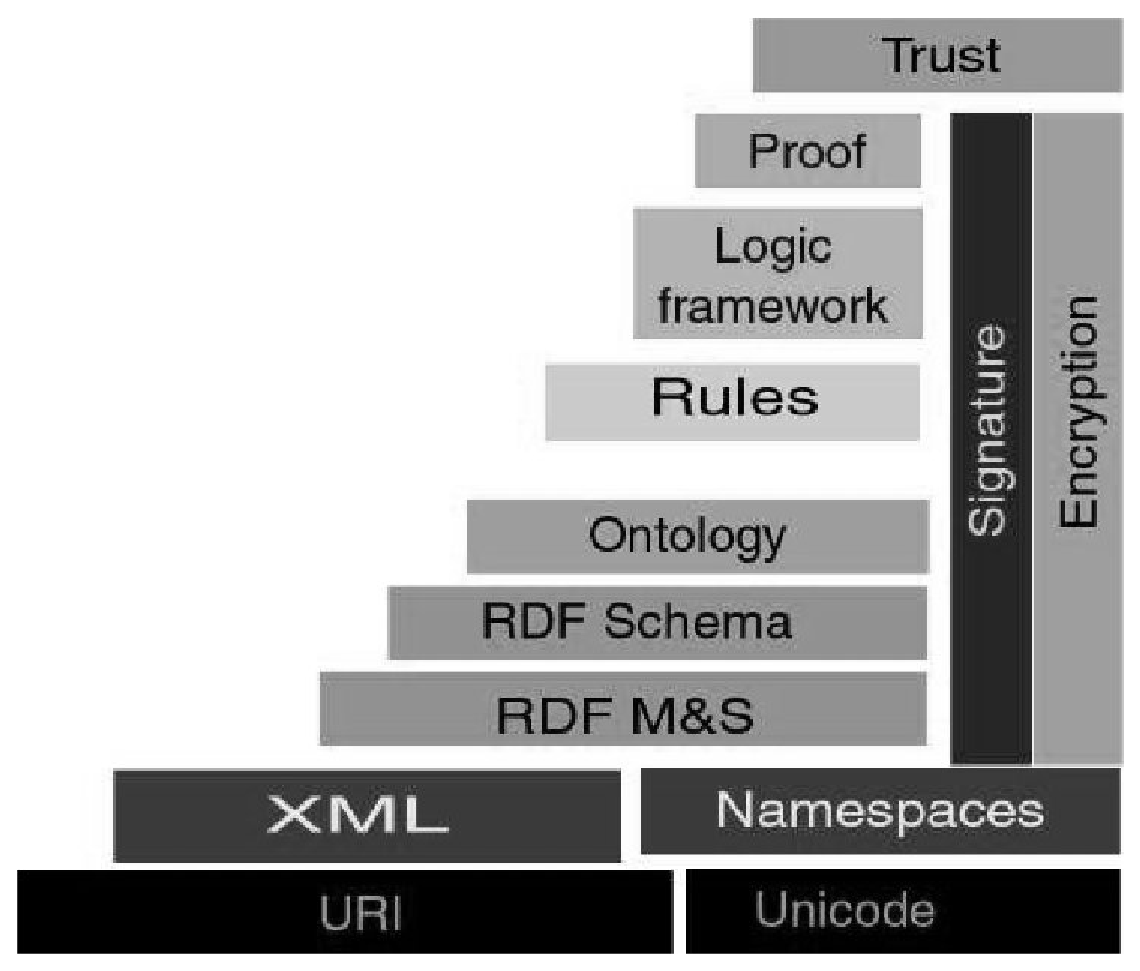
\includegraphics[width=10cm]{images/sw-stack-2002}
\caption{Arquitectura Web Semántica 2002.}
\label{fig:stack-2002}
\end{figure}

A continuación se explica someramente la intención de cada una de las capas y el por qué
de su presencia:
\begin{description}
\item[\gls{URI}/\gls{IRI}-Unicode.] Para dar un soporte estándar a una tecnología existen
dos factores fundamentales: nombrado e identificación única de cada uno de los
recursos y codificación de los mismos. Por esta doble razón aparecen los \textit{Unified
Resource Identifier} y la codificación estándar Unicode, implementada principalmente en UTF-8.
\begin{example}
URI: protocolo:dirección:directorio:recurso, \url{http://www.josemalvarez.es/foaf.rdf}
\end{example}

\item[\gls{XML}~\cite{XML11}.] Lenguaje extensible de marcas (\textit{eXtensible Markup
Language}), es un formato estándar creado para la estructuración de datos, en la actualidad 
se encuentra regulado por el \gls{W3C} que es el encargado de realizar las distintas
especificaciones y versiones desde Febrero de 1998. XML está basado en \gls{SGML}
(\textit{Standard Generalized Markup Language}, ISO 8879) que ya había sido establecido
en 1986. El uso principal de XML es la estructuración de datos, pero en general es utilizado por todas
aquellas aplicaciones informáticas en las que se pueda representar la información jerárquicamente.
El lenguaje XML es en sí mismo un metalenguaje utilizado ampliamente para definir otros
lenguajes. Consta entre otros, de elementos y atributos. Su orden y jerarquía
son los encargados de formar el lenguaje definido con XML. No se dispone de etiquetas predefinidas, como podría ser \gls{HTML}, siendo el 
usuario el responsable de definir un conjunto de elementos con sus
etiquetas asociadas, la semántica de los documentos es proporcionada por la aplicación que use
esos datos. Para definir la estructura de un documento XML, es decir, una 
gramática que indique el orden de los elementos y su jerarquía, se consigue de dos formas utilizando:\linebreak 1) \gls{DTD} o 2) \gls{XML Schema}~\cite{XMLSchema}.

Es importante resaltar que un documento bien formado no es lo mismo que un documento
válido, un documento estará bien formado cuando siga las reglas sintácticas de
formato XML, mientras que un documento será válido si todos sus elementos están en orden correcto de anidación y está bien formado. 
La utilización de XML resulta de interés en base a alguna de las razones siguientes:
\begin{itemize}
\item Estándar para el intercambio de datos.
\item Facilidad de uso.
\item Legibilidad.
\item Implantación.
\item Extensibilidad.
\item Separación entre formato y contenido.
\item Tratamiento multiplataforma.
\item Es libre, especificaciones disponibles. 
\end{itemize}

\begin{figure}[!htbp]
\centering
\lstinputlisting[language=XML]{examples/events.xml}
\caption{Ejemplo de fichero XML.}
\label{fig:ejemplo-xml}
\end{figure}

Como aplicación práctica de XML, ver Figura~\ref{fig:ejemplo-xml}, y debido a la necesidad de tratamiento
automático para diferentes fines (formatos de presentación, transformación de un
vocabulario a otro, etc.) hay que destacar \gls{XSL}~\cite{XSL} para la generación del
contenido a partir de un documento XML de una manera rápida, sencilla y eficaz, cuyo objetivo principal es presentar al usuario final un 
interfaz del documento más comprensible con el que pueda realizar un tratamiento de la información contenida en él de una forma más
asequible, sin necesidad de conocer el formato XML.

\begin{figure}[!htbp]
\centering
	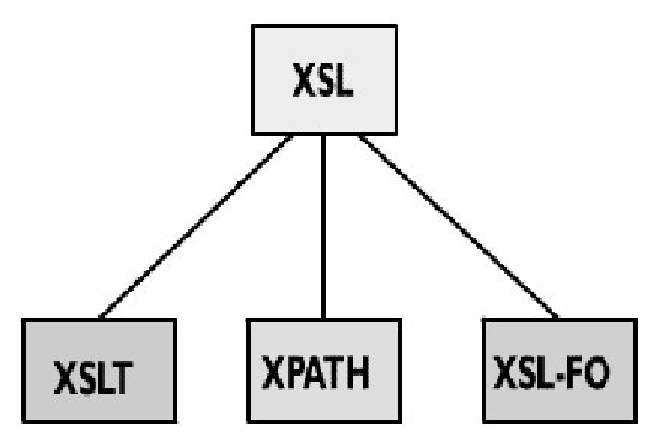
\includegraphics[width=6cm]{images/xsl}
\caption{Componentes de XSL.}
\label{fig:xsl}
\end{figure}

Por ello desde el consorcio \gls{W3C} se optó por realizar la especificación XSL con
el objetivo de presentar un modelo para el procesamiento de la información
almacenada en formato XML. La especificación redactada por el consorcio web para la transformación del contenido XML
se denomina XSL, se encarga de definir una hoja de estilo con la cual se transforma el fichero
XML en otro formato, teniendo en cuenta que la información en XML se almacena de forma
jerarquizada, con la definición de XSL se pretende poder presentar al usuario dicha información
en otros formatos estructurados como pueden ser: HTML, \gls{PDF}, etc., XSL es una especificación, pero 
el lenguaje del que hace uso para la realización de la transformación es XSLT con sintaxis de XPath~\cite{XPath}.

En \gls{XSLT} se define cómo se ha de realizar la transformación del documento XML y no
cuándo, así la transformación del documento se realiza en distintos pasos: 
\begin{itemize}
    \item Generación de un árbol a partir del fichero fuente de XML, esto se
    realiza mediante un procesador que analiza el documento, realizando al mismo tiempo una validación sintáctica del
mismo.
\item Procesamiento del árbol generado construyendo un nuevo árbol con la
información procesada, el recorrido del árbol generado se realiza en preorden, con la posibilidad de variar el tipo de recorrido, es importante tener en cuenta
el orden de evaluación de los nodos del árbol para así poder aplicar las
plantillas correctamente. 
\end{itemize}

El principal uso de XSLT como ha quedado patente en la introducción, es la transformación
de documentos XML para generar contenido web, lógicamente esto no aportaría demasiada potencia
a este lenguaje si solo sirviera para generar contenido web estático, en cambio usando
este lenguaje se genera contenido dinámico aplicando distintas reglas, como ejemplo se
podría obtener de una base de datos un fichero XML y con dicho fichero y una transformación
apropiada generar una página dinámica con contenidos auto-actualizables cada cierto tiempo, otro 
ejemplo de aplicación podría ser la conversión de un programa escrito en un lenguaje a otro, definiendo las reglas correctas. 
XSLT utiliza también \gls{XPath}, ver Figura~\ref{fig:xsl-example}, que es una especificación
para el acceso a los valores de los distintos nodos del árbol generados a partir del procesamiento
del fichero XML. 

\begin{figure}[!hbp]
\centering
\small
\lstinputlisting[language=XML,basicstyle=\scriptsize]{examples/events.xsl}
\caption{Ejemplo de hoja de estilo XSL.}
\label{fig:xsl-example}
\end{figure}


\item[\gls{XML Schema}~\cite{XMLSchema}.] En primer lugar es interesante diferenciar las dos
tecnologías establecidas para la definición de la estructura de un documento
XML: \begin{inparaenum}
     \item \textit{Document Type Definition} (\gls{DTD}) es un vocabulario para definir las
     reglas de construcción de un documento XML.     
     \item XML Schema: Vocabulario XML utilizado para definir otros vocabularios
     XML.  
     \end{inparaenum}

El incremento en el uso de \gls{XML} hace necesario la utilización de tecnología para poder
expresar la estructura del documento y así proceder a su validación. Aunque en principio el objetivo de ambos es el mismo: 
definir vocabularios XML para poder validarlos sintácticamente e imponer distintos tipos de 
restricciones como de cardinalidad o integridad, cada uno presenta unas características diferentes 
lo que supone que escoger entre uno u otro implique realizar un estudio de lo que se pretende desarrollar.
También disponemos de herramientas que nos permiten realizar la transformación de uno a
otro pero sólo en el sentido de DTD a XML Schema. Se puede pensar que XML Schema es el
sucesor de las DTD.

La utilización de XML Schema, ver Figura~\ref{fig:xsd-example}, se apoya en diferentes características que hacen
que su uso sea interesante en el ámbito de la Web Semántica:
\begin{itemize}
\item Espacios de nombres, permite utilizar los mismos identificadores en el
mismo documento, evitando así la ambigüedad.
\item Esquema, es la estructura que va a presentar el vocabulario XML construido, con
sus distintos elementos y atributos así como con las validaciones que sean
necesarias.
\item Documento instancia,  documento XML creado con una estructura
definida en un XML Schema y contra el cual se ``valida''.
\end{itemize}

Las razones que pueden llevar a elegir XML Schema son, entre otras, las siguientes:
\begin{itemize}
  \item Utiliza sintaxis XML.
  \item Perfectamente documentado.
  \item Define los elementos y atributos que pueden aparecer en un documento instancia.
  \item Establece la jerarquía y orden de los distintos elementos.
  \item Creación de distintos tipos genéricos.
  \item Extensible.
  \item Inclusión de documentos externos.
  \item Expresividad.
  \item Posibilidad de documentación.
  \item Tipos de datos simples, complejos, derivados.
  \item Expresión de restricciones de integridad y cardinalidad.
  \item Reutilización de tipos por extensión o restricción.
  \item \ldots  
\end{itemize}


\begin{figure}[!htbp]
\centering
\lstinputlisting[language=XML,basicstyle=\tiny]{examples/events.xsd}
\caption{Ejemplo de XML Schema.}
\label{fig:xsd-example}
\end{figure}


La utilización de XML Schema es crítica en los servicios web basados en \gls{WSDL}~\cite{WSDL20} y \gls{SOAP}~\cite{SOAP11} y 
está muy asentada en entornos de desarrollo basados en Java a través de herramientas como \gls{JAXB}.

\item[\gls{RDF}~\cite{RDF}.] \textit{Resource Description Framework}, se encarga
de describir los recursos, añadiéndoles la metainformación necesaria en
un formato procesable. En la siguiente Sección~\ref{rdf} se aborda la descripción de
RDF de manera más extensa.

\item[Ontologías:] Los documentos etiquetados constituyen una gran cantidad
de información disponible para utilizar por la máquina. Están disponibles los datos, pero
todavía no hay capacidad semántica, es necesario construir un modelo donde ``encajar''
esos datos. Para añadir la componente semántica mediante ontologías, ver Sección
\ref{ontologias}, se pueden utilizar diferentes lenguajes, cuyo estudio se 
abordará en la Sección~\ref{lenguajes}.

\item[Capas superiores:] La arquitectura propone diferentes niveles en los
que se colocan las reglas y la lógica, debido a su complejidad todavía es precipitado definirlas por completo y las discusiones se mantienen
abiertas en grupos de trabajo del \gls{W3C} como el \gls{RIF}~\cite{rif-core}. 
Los módulos transversales de ``firma''~\cite{XML-dsig} y 
``encriptación''~\cite{XML-enc} están definidos y se
pueden encontrar como recomendaciones del W3C.

\end{description}

Aunque las ventajas de un diseño basado en capas está sobradamente demostrado en
bibliografía de ingeniería del \textit{software}, hay que resaltar que esta primera
aproximación ha sido modificada con el objetivo de recoger la realidad de la
arquitectura para la Web Semántica. Hay que tener en cuenta que la primera
versión propuesta por \textit{Tim Berners Lee} (web XML) ofrecía una visión ideal
que contemplaba todas las partes implicadas, pero que no tenía el efecto experiencia
de la construcción de aplicaciones y de los posibles problemas que se podrían
encontrar. Por ello, esta arquitectura ha sido rediseñada planteando un modelo
más cercano a la realidad, al menos de las aplicaciones y problemas, siendo también 
conocida como las ``dos torres''~\cite{kifer05} (web RDF), ver Figura~\ref{fig:stack-2005}.

\begin{figure}[!htbp]
\centering
	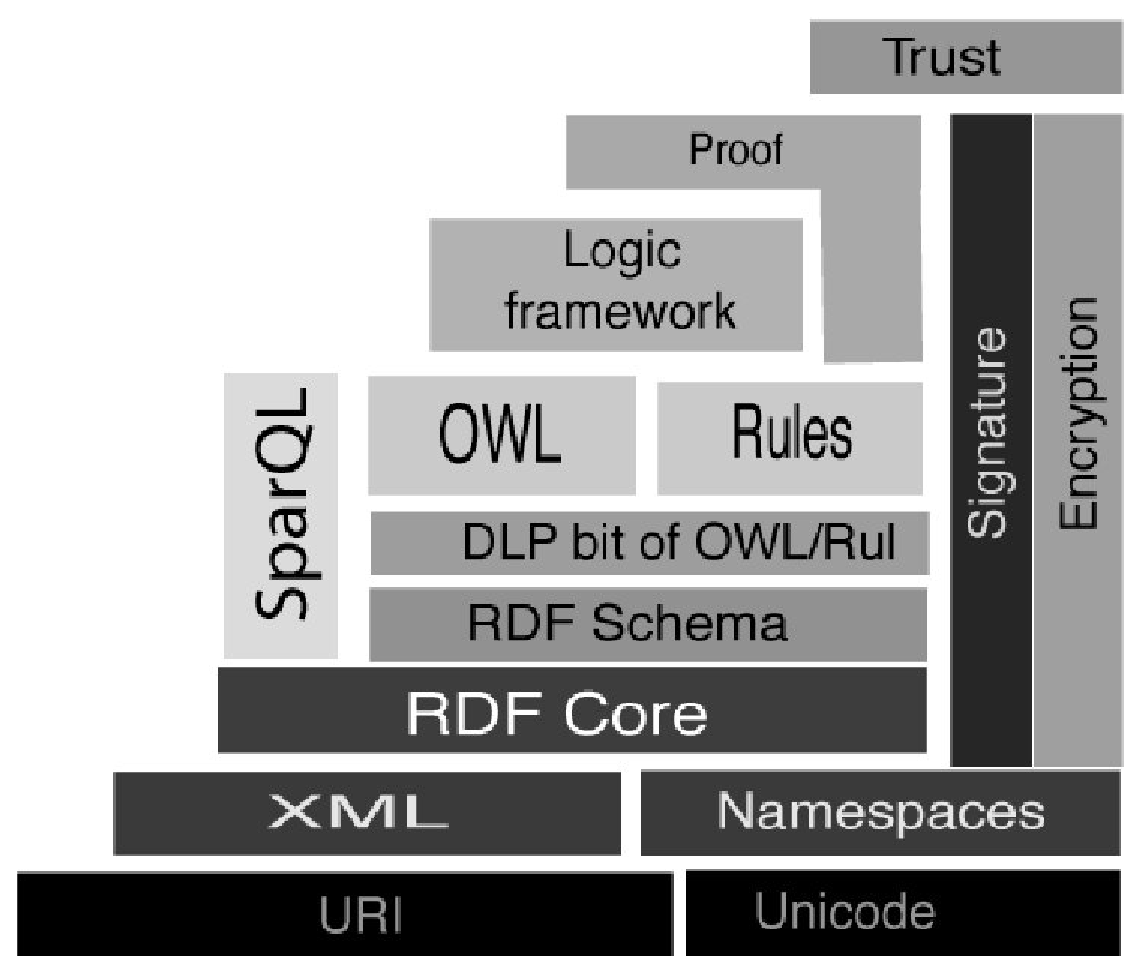
\includegraphics[width=10cm]{images/sw-stack-2005}
\caption{Arquitectura Web Semántica 2005.}
\label{fig:stack-2005}
\end{figure}

La propuesta de cambio surge porque la Lógica Descriptiva, que utiliza \gls{OWL}, no
tiene un poder expresivo suficiente para solucionar el problema de la
representación de conocimiento y razonamiento en la Web Semántica. OWL no puede
tratar con información de una forma dinámica, no tiene predicados \textit{n-arios}, no
soporta símbolos de función, etc. De ahí que se valorara la posibilidad de extender las bases
de conocimiento en OWL con reglas para aumentar la expresividad de los modelos y
ganar en capacidad de inferencia.

Las reglas, en programación lógica como PROLOG, tienen una larga tradición en
las ciencias de la computación y se llevan estudiando desde hace más de 20 años, 
sin embargo, la extensión de OWL con reglas no es una tarea sencilla. En general, las reglas 
están basadas también en un subconjunto de la lógica de primer orden, la
lógica \textit{Horn}, aunque su semántica formal es diferente, no está basada en teoría de modelos. La diferencia fundamental, aparte del tratamiento
de la negación y cuestiones de expresividad, tiene que ver con OWL, ya que, 
debido a su semántica de primer orden, utiliza la hipótesis de mundo abierto,
mientras que las reglas habituales de programación lógica utilizan mundo cerrado. 

La extensión más conocida de OWL en este sentido es \gls{SWRL}~\cite{Swrl}, que permite claúsulas
Horn como axiomas en las bases de conocimiento en OWL. Este lenguaje mantiene
el mundo abierto de OWL, pero penaliza en rendimiento debido a su alto coste computacional.

Debido a esta serie de problemas, se ha sugerido la opción de separar ontologías y
reglas (lógica descriptiva y programación lógica) y utilizar cada tecnología en los escenarios pertinentes y apropiados. La combinación entre ambos, un objetivo verdaderamente ambicioso de la Web Semántica, 
ya no sería mediante la extensión de OWL con algún tipo de formalismo para la expresión de reglas, sino mediante la construcción
de un interfaz lógico que permita desde las reglas utilizar información definida
en las ontologías, y desde éstas, información inferida por el
comportamiento de los sistemas de reglas.

Destacar la aparición del lenguaje de consulta para RDF, \gls{SPARQL}~\cite{Sparql} y su última
versión SPARQL 1.1, creado por la necesidad de disponer de un lenguaje de acceso a los recursos
definidos en forma de grafo y con una semántica definida~\cite{Perez:2009:SCS:1567274.1567278}. El modelo semántico~\cite{citeulike:1556975} 
proporcionado por RDF permite tratar cualquier recurso como una entidad con descripción asociada. No obstante, el uso de RDF no es
suficiente para la elaboración de modelos de dominio más ricos y descriptivos, razón por la cual surge un lenguaje como OWL que apoyado sobre el modelo de RDF
permite realizar formalizaciones utilizando diferentes lógicas (principalmente \textit{Description Logics}).

\subsubsection{Lenguajes para la Web Semántica: Creando ontologías}\label{lenguajes}
La construcción de una base de conocimiento~\cite{GruberOnto} utilizando ontologías puede
realizarse con distintos lenguajes y diferentes grados de expresividad lógica~\cite{HoPa10a,Kifer:1989:FHL:66926.66939}.
La selección de la lógica apropiada para la modelización de nuestra base de
conocimiento no es una cuestión sencilla y deben contemplarse diferentes
factores: grado de computabilidad, decidibilidad, soporte de los razonadores, etc. Todos ellos determinarán la lógica a utilizar ya que no se puede señalar arbitrariamente que se debe utilizar un nivel lógico cuando no es necesario para
el modelo formal.
\subsubsection{RDF}\label{rdf}
El primer lenguaje que se encuentra para la creación de ontologías es \gls{RDF}
(\textit{Resource Description Framework}) como soporte básico a la par que potente, 
para añadir semántica a los recursos (documentos entre otros). La primera observación 
a realizar es la distinción entre: 1) modelo de datos, basado en
tripletas Sujeto-Predicado-Objeto y 2) formato de datos, puede utilizar RDF/XML (normativo)
como formato para la serialización del modelo.

El modelo de datos de RDF utiliza tripletas, ver Figura~\ref{fig:rdf-model}, encargadas de describir recursos:
\begin{description}
\item[Sujeto:] recurso sobre el que vamos a realizar una afirmación. Están
identificados de forma única a través de URIs, por ejemplo: Yo.
\item[Predicado:] es la afirmación sobre el sujeto, por ejemplo: ``tengoNombre''.
\item[Objeto:] valor del predicado para este sujeto, por ejemplo: ``Jose María''@es.
\end{description}

\begin{figure}[!htbp]
\centering
	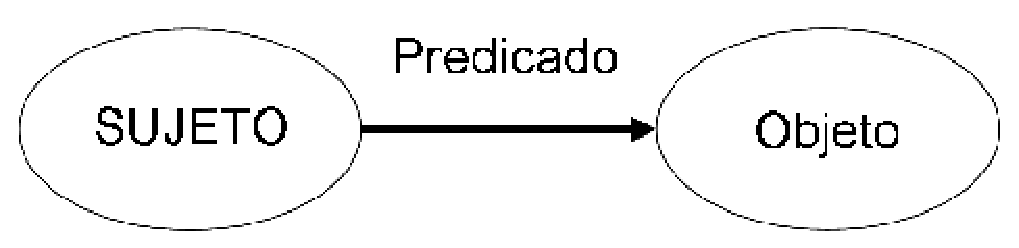
\includegraphics[width=10cm]{images/rdf-model}
\caption{Modelo de tripletas RDF.}
\label{fig:rdf-model}
\end{figure}

Usando RDF pueden realizarse afirmaciones simples sobre ``cosas'': ``Este
documento de memoria tiene de creador'' a ``Jose María Alvarez'' puede expresarse en
RDF usando la tripleta (memoria, ``tieneCreador'', ``Jose María Alvarez''). 
A su vez  se pueden generar nuevas tripletas (memoria, ``tieneFecha'',
``Enero 2012'') o (memoria, ``tieneFormato'', ``PDF''), generando así un
modelo semántico simple pero perfectamente válido. Si se le añade el uso de colecciones y 
la capacidad de ``reificación'' (afirmaciones sobre otras
afirmaciones) se conseguirá una capacidad de expresión muy potente asentada en un
sencillo lenguaje. En cuanto, a la serialización de RDF o su formato, existen diferentes estándares perfectamente válidos para su tratamiento automático por las máquinas y más o
menos amigables para los humanos. 
\begin{itemize}
  \item \gls{RDF/XML}~\cite{rdf-syntax} formato estándar y normativo por excelencia, ver Figura~\ref{fig:rdf-n3}. 
\begin{figure}[!htbp]
\centering
  \begin{lstlisting} 
<rdf:RDF xmlns:rdf="http://www.w3.org/1999/02/22-rdf-syntax-ns#"
  xmlns:rdfs="http://www.w3.org/2000/01/rdf-schema#"
  xmlns:dc="http://purl.org/dc/elements/1.1/">
    <rdf:Description rdf:about="http://petra.euitio.uniovi.es/~i1637566/">
      <dc:creator>Jose M. Alvarez</dc:creator>
    </rdf:Description>
</rdf:RDF>  
  \end{lstlisting} 
\caption{Ejemplo de tripletas de RDF en RDF/XML.}
\label{fig:rdf-n3}
\end{figure}  

\item Otros como: \gls{RDFa}~\cite{rdfa-primer}, \gls{Turtle}~\cite{turtle-syntax}, \gls{N3}~\cite{n3-syntax} ,\gls{RDF}/\gls{JSON}~\cite{rdf-json} o RDF binario~\cite{rdf-binario}.   
\begin{figure}[!htbp]
\centering
  \begin{lstlisting} 
@prefix dc <http://http://purl.org/dc/elements/1.1/>
<http://petra.euitio.uniovi.es/~i1637566/> dc:creator "Jose M. Alvarez"
  \end{lstlisting}
\caption{Ejemplo de tripleta de RDF en N3.}
\label{fig:rdf-n3}
\end{figure}


 \end{itemize}

En definitiva, RDF provee un mecanismo muy útil para describir recursos que
no realiza presunciones sobre un dominio y capaz de representar a cualquiera
de ellos. La declaración de propiedades (atributos) y su valor semántico se definen
en el contexto de RDF con RDFS (\textit{\gls{RDF Schema}}). RDFS se construye por
encima de RDF y sirve, no solo para definir las propiedades del recurso, sino también
el tipo de recurso. Se pueden crear \textit{clases de recursos}, restringir
combinaciones de las clases, de las relaciones, además de ser el primer nivel de
semántica que permite detectar estas aserciones. RDFS está basado en el
metamodelado de objetos, el principal problema lo constituye la posibilidad de que una
misma clase pueda desarrollar un doble rol de clase o de instancia, aunque se puede utilizar como
un lenguaje de ontologías desde el punto de vista del manejo de clases, propiedades, rangos y dominios sobre propiedades. 
La posibilidad de generación de jerarquía de conceptos es un lenguaje muy limitado para la expresión de datos en
detalles y no asegura la computabilidad. Es interesante conocer algunos de los vocabularios RDF, especialmente
con el advenimiento de la iniciativa de \linkeddata, que se han creado con distinto propósito, con muy buena 
acogida en la comunidad de Internet y cada día con un uso más extendido: 

\begin{description}
\item[\textit{Dublin Core}.] Vocabulario RDF con las propiedades más comunes y semántica bien definida para el etiquetado de cualquier documento.

\begin{itemize}
  \item Cada etiqueta es opcional y puede estar repetida. Un documento no
  necesita tener resumen y puede tener varios autores.
  \item La mayoría de etiquetas tienen cualificadores para refinar (nunca extender) su significado.
Por ejemplo, la etiqueta ``fecha'' tendrá como cualificadores ``de publicación'',
``de creación'', etc.
\item Principio del Uno-a-Uno. Los metadatos se refieren a un documento
concreto, no a lo representado. 
\item  Principio del \textit{Dumb-down}. Si no se procesan las restricciones al
significado de las \linebreak propiedades, estas deben seguir proporcionando información
útil. Se pierde nivel de detalle, pero la información sigue siendo válida.
\item Las buenas prácticas de uso para una etiqueta determinada pueden variar por
el contexto. El creador no puede dar por supuesto que serán interpretadas exclusivamente por
una máquina, esto impondrá algunas restricciones a cómo se construyen los
metadatos, pero no se debe eludir que el requisito fundamental de
estos es su utilidad para descubrir información.
\end{itemize}

Usando estos principios, \textit{Dublin Core} se impuso el objetivo de lograr un lenguaje
de etiquetado: simple y fácil de mantener, semántica esencial y de significado común, alcance internacional y extensible.
Se pueden establecer dos escenarios muy habituales en el uso de este vocabulario:
\begin{enumerate}
  \item En los metaelementos presentes en \gls{HTML} y \gls{XHTML}, ver Figura~\ref{fig:html-dc-example}.

\begin{figure}[!htbp]
\centering
  \begin{lstlisting} 
  <head>
<title>Dublin Core Metadata Initiative (DCMI)</title>
<link rel="schema.DC" href="http://purl.org/dc/elements/1.1/" />
<meta name="DC.title" content="Dublin Core Metadata Initiative (DCMI) Home Page" />
<meta name="DC.description" content="The Dublin Core Metadata Initiative is an open forum . . . metadata standards and practices." />
<meta name="DC.date" content="2011-10-01" />
<meta name="DC.format" content="text/html" />
<meta name="DC.contributor" content="Dublin Core Metadata Initiative" />
<meta name="DC.language" content="en" />
</head>  
 \end{lstlisting} 
\label{fig:html-dc-example}
\caption{Ejemplo de \textit{Dublin Core} en HTML/XHTML.}
\end{figure}
 
\item En documentos RDF propiamente dichos como metadatos de los recursos. A
continuación, se puede ver en la Figura~\ref{fig:rdf-dc-example} el uso de \textit{Dublin Core} en combinación con \gls{RSS}.

\begin{figure}[!htbp]
\centering
\begin{lstlisting}
<rdf:RDF
 xmlns:rdf="http://www.w3.org/1999/02/22-rdf-syntax-ns#"
 xmlns="http://purl.org/rss/1.0/"
 xmlns:dc="http://purl.org/dc/elements/1.1/"
 xmlns:syn="http://purl.org/rss/1.0/modules/syndication/"
 xmlns:taxo="http://purl.org/rss/1.0/modules/taxonomy/"
>
<channel rdf:about="http://dublincore.org">
<title>Dublin Core Metadata Initiative</title>
<link>http://dublincore.org/</link>
<description>Making it easier to find information.</description>
<dc:language>en-us</dc:language>
<dc:rights>1995-2007</dc:rights>
<dc:date>2007-10-01</dc:date>
<items>
<rdf:Seq>
  <rdf:li rdf:resource="http://dublincore.org/news/2007/#dcmi-news-20071001-01" />
  <rdf:li rdf:resource="http://dublincore.org/news/2007/#dcmi-news-20071001-02" />
  <rdf:li rdf:resource="http://dublincore.org/news/2007/#dcmi-news-20071001-03" />
  <rdf:li rdf:resource="http://dublincore.org/news/2007/#dcmi-news-20071001-04" />
</rdf:Seq>
</items>
</channel>

</rdf:RDF>
 \end{lstlisting} 
\label{fig:rdf-dc-example}
\caption{Ejemplo de \textit{Dublin Core} con RDF.}
\end{figure}

\end{enumerate}

\item[\gls{SKOS}-Core~\cite{SKOS-Core}.] Vocabulario RDF utilizado para la representación de conocimiento 
de forma simple a través de conceptos, para ser procesado por máquinas de forma
automática: vocabularios controlados, taxonomías, tesauros, esquemas
conceptuales, glosarios o esquemas categorizados. Algunas de las propiedades de SKOS que 
confieren interés a este vocabulario son las siguientes:
\begin{itemize}
\item Identificación de conceptos a través de URIs.
\item  Etiquetado de conceptos: \textit{prefLabel}, \textit{altLabel},
\textit{prefSymbol}, \textit{altSymbol}, etc.
\item Descripción y documentación (conceptos): \textit{definition}, \textit{example}, \textit{scopeNote},
\textit{version}, \textit{changeNote}, etc.
\item Relaciones entre conceptos: \textit{broader}, \textit{narrower},
\textit{related}, etc. 
\item Indexación: \textit{subject}.
\item Soporte multiling\"{u}e.
\end{itemize}

En la siguiente Figura~\ref{fig:skos} se presenta un ejemplo más completo del
uso de SKOS-Core para la descripción de conceptos:
 
\begin{figure}[!htbp]
\centering
	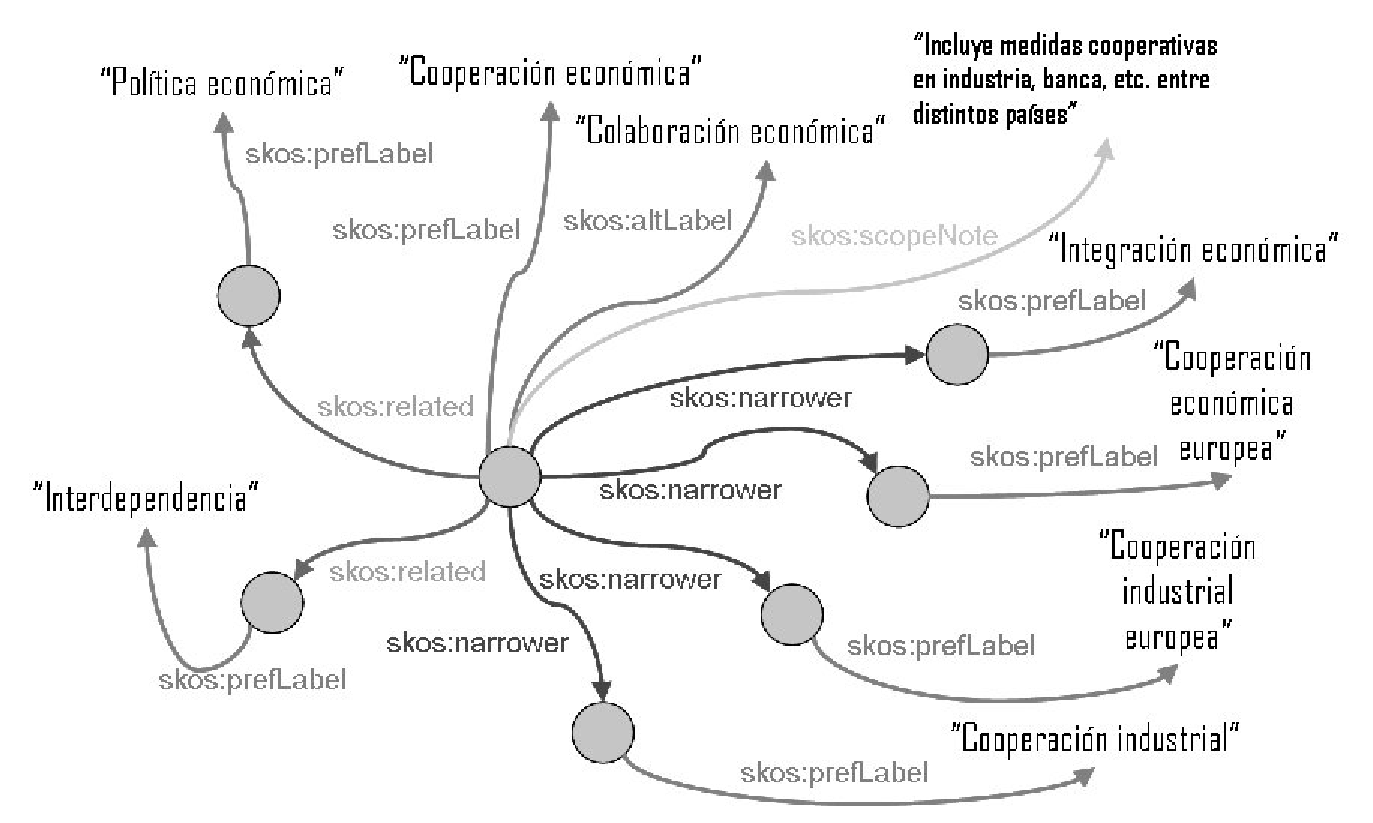
\includegraphics[width=14cm]{images/skos}
\caption{Concepto expresado en SKOS-Core.}
\label{fig:skos}
\end{figure}

Debe puntualizarse que el uso de SKOS-Core está siendo objeto de estudio para la
representación de recursos lexicográficos~\cite{Milin} desde un punto de vista de la
lingüística y como un avance tecnológico en este campo.

\item[\gls{FOAF} y \gls{DOAP}.] Vocabularios RDF para definir personas y amistades (\textit{Friend Of A Friend}), ver Figura~\ref{fig:foaf-example}, o 
proyectos (\textit{Description Of A Project}), 
ver Figura~\ref{fig:doap-example}. Cada vez hay un mayor interés por este tipo de tecnologías y algunos proyectos de gran envergadura como 
Apache o RDF Ohloh~\cite{Ferndez08rdfohloh}, que incluyen muchos subproyectos, programas, etc., utilizan estas
descripciones semánticas para cada módulo.

\begin{figure}[!htbp]
\centering
  \begin{lstlisting}
<#me> a foaf:Person;
	foaf:family_name "Alvarez";
	foaf:givenname "Jose";
	foaf:homepage <http://josemalvarez.es>;
	foaf:knows _:bnode2016979200;
	foaf:mbox_sha1sum "0d1d9ad2de64fd900d03c18e3d2608171832d155";
	foaf:nick "chema";
	foaf:phone <tel:+34-666-714-721>;
	foaf:schoolHomepage <http://www.uniovi.es/inicio/>;
	foaf:title "Sr.";
	foaf:workplaceHomepage <http://www.weso.es>.

_:bnode2016979200 a foaf:Person;
	rdfs:seeAlso <http://www.di.uniovi.es/~labra/labraFoaf.rdf>;
	foaf:mbox_sha1sum "5fa5d69bac0c1396825c475ec19325ec0ffd5569";
	foaf:name "Jose Emilio Labra".
  \end{lstlisting}
\caption{Ejemplo parcial de documento FOAF en N3.}
\label{fig:foaf-example}
\end{figure}


\begin{figure}[!htbp]
\centering
  \begin{lstlisting}
<http://rdfohloh.wikier.org/project/moldeas/rdf> 
	dct:isFormatOf 	<http://rdfohloh.wikier.org/project/moldeas>;
	a foaf:Document;
	rdfs:label "MOLDEAS's DOAP document serialized in RDF/XML";
	foaf:primaryTopic <http://rdfohloh.wikier.org/project/moldeas>.
	<http://rdfohloh.wikier.org/project/moldeas> dct:updated "2012-01-22T13:02:25Z";
	rdfohloh:ohloh-page <http://www.ohloh.net/projects/moldeas>;
	doap:created "2011-10-14T09:19:11Z";
	doap:description "This work aims to apply the semantic web and 
	    LOD approaches to public procurement notices...";
	doap:download-page <http://code.google.com/p/moldeas/downloads/list>;
	doap:homepage <http://purl.org/weso/moldeas/>;
	doap:name "MOLDEAS";
	doap:programming-language "JavaScript";
	a doap:Project;
	= <http://rdfohloh.wikier.org/project/586667>;
	skos:subject <http://dbpedia.org/resource/Java>, 
	<http://dbpedia.org/resource/JavaScript>.
  \end{lstlisting}
\caption{Ejemplo parcial de documento DOAP en N3.}
\label{fig:doap-example}
\end{figure}

\newpage

\item[\gls{SIOC}.] (\textit{Semantically-Interlinked Online Communities}). Es una ontología desarrollada 
por el equipo de Web Semántica de DERI Galway para describir semánticamente
distintas comunidades \textit{online}. SIOC integra, ver Figura~\ref{fig:sioc-example}, distintos vocabularios RDF con el
objetivo de reutilizar las definiciones ya realizadas en \gls{FOAF}, \gls{SKOS},
\gls{RSS} o \textit{Dublin Core}. Se ha empleado con éxito en distintas aplicaciones para gestionar y
describir toda la información disponible de las comunidades \textit{online}: listas de correo (SWAML~\cite{Sergio}), 
foros, etc.
 

\begin{figure}[!htbp]
\centering
  \begin{lstlisting}
<rdf:RDF
  xmlns:sioc='http://rdfs.org/sioc/ns#'
  xmlns:rdf='http://www.w3.org/1999/02/22-rdf-syntax-ns#'
  xmlns:dc='http://purl.org/dc/elements/1.1/'
  xmlns:mvcb='http://webns.net/mvcb/'
>
  <sioc:Site rdf:about="http://groups.google.com/group/sioc-dev">
    <sioc:host_of>
      <sioc:Forum rdf:about="http://swaml.berlios.de/demos/sioc-dev/index.rdf#SIOC-Dev">
        <dc:description>SIOC development mailing list</dc:description>
        <mvcb:errorReportsTo rdf:resource="http://swaml.berlios.de/bugs"/>
        <sioc:container_of rdf:resource="http://swaml.berlios.de/demos/sioc-dev/2006-Dec/post-419.rdf"/>
        <dc:date>2007-06-18</dc:date>
        <dc:title>SIOC-Dev</dc:title>
        <mvcb:generatorAgent rdf:resource="http://swaml.berlios.de/doap.rdf"/>
        <sioc:has_host rdf:resource="http://groups.google.com/group/sioc-dev"/>
        <sioc:has_subscriber rdf:resource="http://swaml.berlios.de/demos/sioc-dev/subscribers.rdf#s26"/>
      </sioc:Forum>
    </sioc:host_of>
  </sioc:Site>
</rdf:RDF>
  \end{lstlisting}
\caption{Ejemplo de descripción con SIOC.}
\label{fig:sioc-example}
\end{figure}

\item[\gls{RSS}.] Existen diferentes versiones y definiciones de este vocabulario RDF: \textit{Rich Site Summary} (RSS 0.91), XML; 
\textit{RDF Site Summary} (RSS 0.9 y 1.0), RDF; \textit{Really Simple Syndication} (RSS 2.0). La definición
realizada en el \gls{W3C} es la siguiente:

\begin{Frame}
\textit{Vocabulario RDF basado en XML que permite la catalogación de información (noticias y eventos) 
de los usuarios. Los archivos RSS contienen metadatos sobre fuentes de información especificadas 
por los usuarios, cuya función principal es notificar de forma automática cualquier cambio que se realice 
en esos recursos de interés.}
\end{Frame}

% \begin{figure}[!htb]
% \centering
% \lstinputlisting[language=XML]{examples/rss.rss}
% \label{fig:rss-example}
% \caption{Ejemplo de canal RSS.}
% \end{figure}

\end{description}

En resumen, se dispone de un lenguaje muy útil y sencillo para describir recursos (RDF) y 
un esfuerzo en forma de vocabulario para la definición de recursos más detallada (RDFS) pero incompleto. 
Por ello, a continuación, se expondrán algunos de los lenguajes más completos que han surgido para 
intentar mejorar los puntos débiles de esta primera aproximación para la expresión de modelos semánticos. En cuanto
a vocabularios RDF existen una infinidad~\cite{common-vocabularies} de ellos para ser utilizados en distintos contextos que han sido
enormemente impulsados por la corriente \linkeddata y \opendata.
%Avoiding too many floats 
%\clearpage

\subsubsection{OIL}
El \textit{Ontology Inference Layer}~\cite{Fensel01oil:an} (\gls{OIL}) desarrollado en el proyecto Europeo 
\textit{OntoKnowledge} está construido por encima de \gls{RDF} y RDFS utilizando muchos de sus constructores e intentando
mantener la compatibilidad hacia atrás. OIL provee características de modelado
basada en lógica de marcos~\cite{Kifer:1989:FHL:66926.66939} y \textit{Description Logic}~\cite{baader03description}.

La importancia de OIL reside en la unificación de:
\begin{itemize}
\item \textit{Description Logic}, heredando su semántica formal y la capacidad
de razonamiento efectivo (FaCT++, Racer o Pellet).
\item Sistemas basados en marcos, incorpora las características básicas de
modelado basado en marcos (conceptos, superclases, atributos, etc.).
\item Estándares web, construido sobre RDF y RDFS y utilizando como formato de
intercambio de datos XML.
\end{itemize}

Las ontologías creadas con OIL distinguen distintos meta niveles, con el
objetivo de proporcionar distintos niveles de servicio que pueden ser válidos para un
gran número de ontologías y aplicaciones:
\begin{description}
\item[Primer meta nivel:] también conocido como \textit{definición de ontologías}, en la
cual se proveen las definiciones de ontología, terminología que debería ser
instanciada para definir un vocabulario estructurado con la semántica adecuada.
\item[Segundo meta nivel:] conocido como ``meta meta'' nivel o \textit{contenedor de
ontologías}, describe las características de la ontología tales como autor,
nombre, ámbito, etc. Las anotaciones de este nivel se hacen mediante
\textit{Dublin Core}.
\end{description}

La capacidad de razonamiento es otra de las características importantes de OIL, que no estaba presente en RDF. Habitualmente esta capacidad se utiliza
para realizar las operaciones de clasificación, validación de consistencia e inferencia de nuevo conocimiento de acuerdo a distintos 
niveles de expresividad: 

\begin{description}
\item[Core OIL:] prácticamente compatible con RDFS exceptuando la capacidad de
``reificación''.
\item[Standard OIL:] lenguaje que captura las primitivas y constructores necesarios para
construir modelos semánticos con capacidad de inferencia.
\item[Instance OIL:] inclusión de ``instancias''.
\item[Heavy OIL:] capacidades extras de representación y razonamiento.
\end{description}

% 
% \begin{figure}[htb]
% \centering
% 	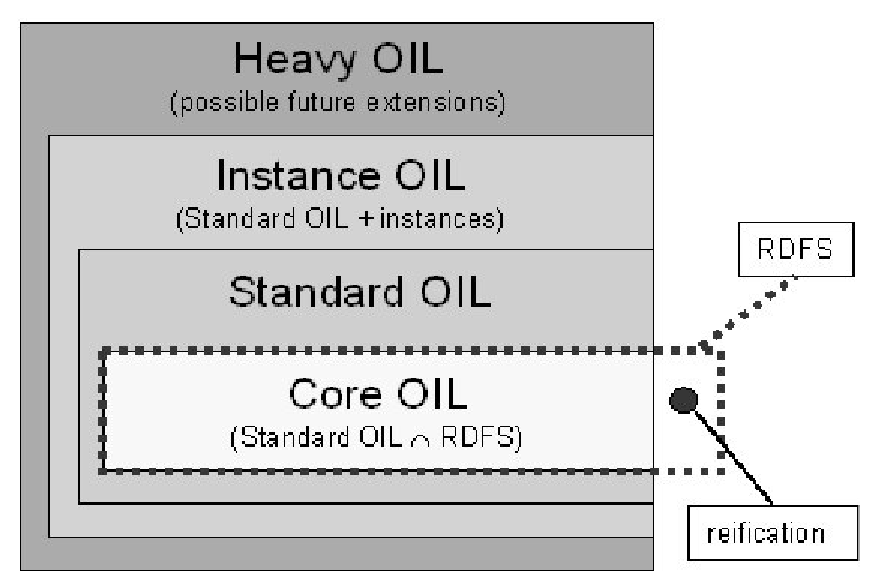
\includegraphics[width=10cm]{images/oil}
% \caption{Niveles de expresividad OIL.}
% \label{fig:oil}
% \end{figure}

Cabe concluir, por tanto, que las principales ventajas de OIL se resumen en:
1) una aplicación no está obligada a trabajar con un
lenguaje más expresivo de lo necesario; 2) aplicaciones que utilicen la
expresividad más baja pueden añadir aspectos de otras ontologías y 3) aplicaciones con un alto nivel de complejidad pueden utilizar
características de otras más simples. Finalmente, el trabajo realizado en 
OIL tiene su continuación en el siguiente lenguaje de modelado de ontologías \gls{DAML+OIL} 
realizado por la cooperación de iniciativas europeas y americanas.

\subsubsection{DAML+OIL}\label{daml+oil}
\gls{DAML+OIL}~\cite{HM00} es un lenguaje de marcado semántico para recursos web creado por la cooperación de las iniciativas
europeas (OIL) y americanas (DAML-ONT, \gls{DARPA} \textit{Agent Markup Language})
en el desarrollo de ontologías. El objetivo de desarrollo de este lenguaje está
especialmente centrado para la Web Semántica, modelización de dominios concretos,
utilizando los estándares (\gls{XML} y \gls{RDF}) y añadiendo una serie de primitivas de
orientación a objetos (clases, propiedades, axiomas y aserciones),
sistemas basados en marcos y parte de \textit{Description Logic}. Además, 
DAML+OIL da soporte a los tipos de datos de \gls{XML Schema}, separando las instancias
de una clase y de las instancias de tipos de datos. El significado de DAML+OIL
está definido por un modelo semántico estándar basado en las interpretaciones, consistiendo éstas 
en un dominio del discurso y una función de interpretación.

\subsubsection{OWL}\label{owl}
\gls{OWL}, lenguaje de ontologías para la web, sucesor de DAML+OIL, actualmente está
siendo desarrollado por el W3C, su primera versión estable es OWL 1.0, 
aunque ya se ha publicado una nueva versión OWL 1.1~\cite{OWL11} y OWL2~\cite{owl2-primer}.

Como lenguaje para ontologías es una potente herramienta que dota de la
expresividad necesaria para mejorar algunos de los servicios más utilizados en
la red de Internet: búsqueda, manejo del conocimiento, interacción entre agentes
automáticos etc. Desde un punto de vista más formal, OWL está formado por
un conjunto de primitivas o constructores de metamodelado que son el punto de
partida para operaciones más complejas, como las de razonamiento. Actualmente,
aunque las características genéricas de OWL tienen su origen en OIL, se distinguen
al menos 3 versiones de OWL (en su versión 1.0 y 1.1) dependiendo de su expresividad, complejidad y grado
de computabilidad, cada versión superior de OWL contiene a la anterior
($Lite\subset DL \subset FULL$).

\begin{description}
\item[OWL-FULL.] Se pueden utilizar todos los constructores y primitivas
definidos en OWL y no restringe el uso de RDF. Esto implica que no se garantiza
su decidibilidad pero en cambio, como familia de \textit{Description Logics}
posee un gran poder expresivo: tratar clases como instancias, definir
propiedades sobre tipos de datos (\textit{string}, \textit{float}, etc.) .

\item[OWL-DL.] Subconjunto decidible de OWL-FULL, supone la máxima expresividad
computable. Cada modelo realizado en OWL-DL genera directamente un modelo
semántico en \textit{Description Logics}.

\item[OWL-Lite.] Añade restricciones adicionales en el uso de los
constructores de OWL, básicamente se pueden modelar jerarquías con restricciones
sencillas.
\end{description}

% Para advertir a que nivel de expresividad y complejidad se puede trabajar
% dependiendo del lenguaje utilizado se dispone la Figura~\ref{fig:owl-dialects}, extraída del laboratorio OntoText.
% 
% \begin{figure}[htb]
% \centering
% 	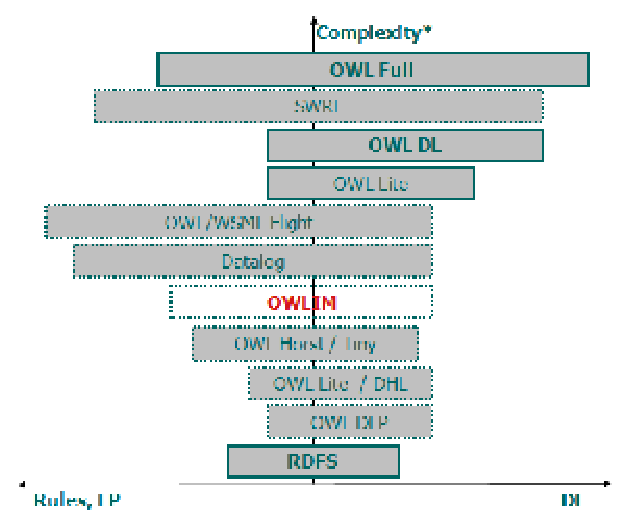
\includegraphics[width=10cm]{images/owl-dialects}
% \caption{Algunos lenguajes para la Web Semántica por OntoText.}
% \label{fig:owl-dialects}
% \end{figure}


Algunas de las características que hacen interesante el uso de OWL en el ámbito
de la Web Semántica son:
\begin{itemize}
  \item Las ontologías en OWL son una serie de axiomas y hechos que pueden
  reutilizar otras ontologías (importándolas). Además, como documento que son
  (serializado en RDF/XML), están identificadas por un URI y tienen asociada cierta metainformación
  (autor, dominio, fecha, etc.) que permite que sean referenciables como
  cualquier otro recurso en la red.
  \item Los axiomas son utilizados para asociar una serie de características
  (descripciones, restricciones, etc.) a las clases y propiedades de la
  ontología. 
\item Los hechos proporcionan información particular de una determinada instancia. 
\end{itemize}

Como ejemplo de utilización de OWL, en su versión DL y con características de OWL2, se presenta una sencilla
ontología, ver Figura~\ref{fig:psydiag}, que modela un sistema de diagnóstico psicológico con capacidad de clasificar individuos
de acuerdo a sus síntomas, ver Figura~\ref{fig:psydiag-axiomas}, con sintaxis Manchester.

\begin{figure}[htb]
\centering
	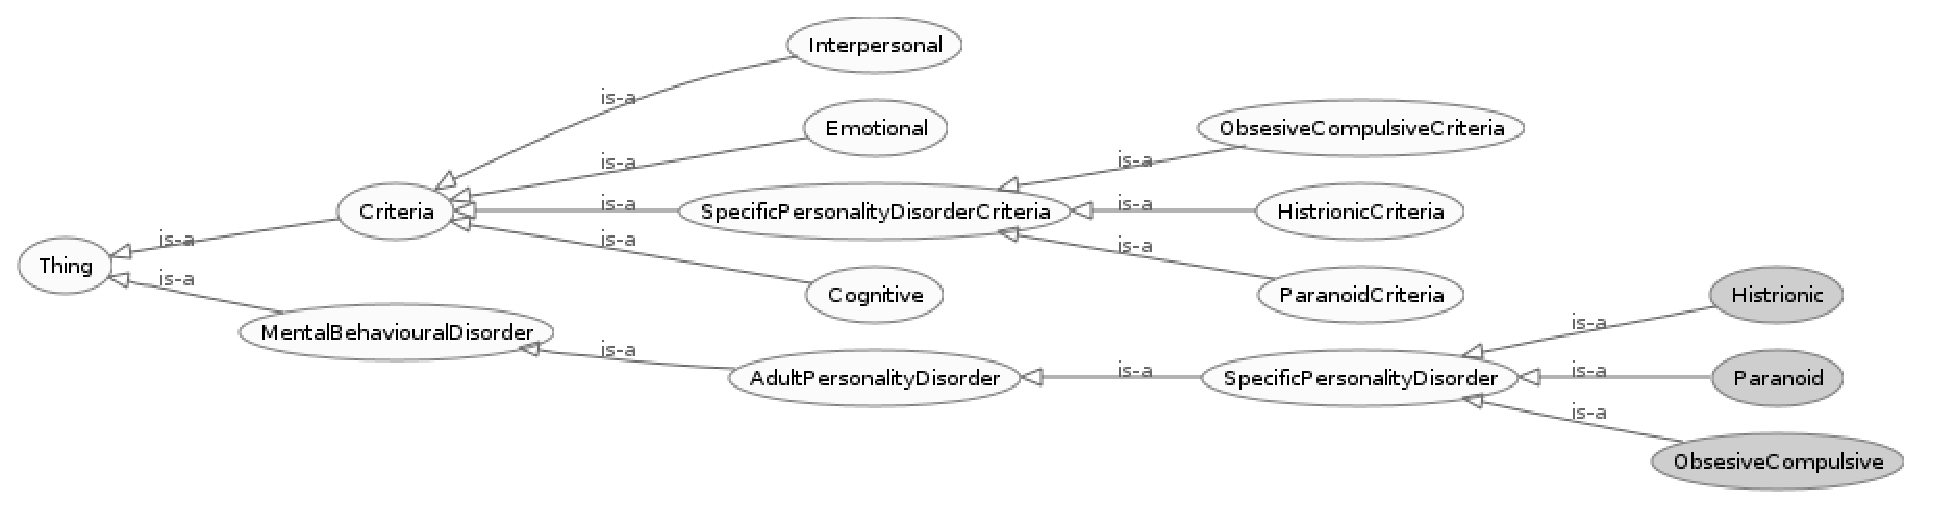
\includegraphics[width=16cm]{images/psydiag}
\caption{Ontología de ejemplo en OWL2 para diagnóstico psicológico.}
\label{fig:psydiag}
\end{figure}


\begin{figure}[htb]
\centering
 \begin{lstlisting} 
Class: <http://example.org/psydiag.owl/Histrionic>

    EquivalentTo: 
        <http://example.org/psydiag.owl/has-criteria> min 3
	      <http://example.org/psydiag.owl/HistrionicCriteria>,
        (not (<http://example.org/psydiag.owl/has-criteria> some 
	      <http://example.org/psydiag.owl/ObsesiveCompulsiveCriteria>))
         and (not (<http://example.org/psydiag.owl/has-criteria> some 
	      <http://example.org/psydiag.owl/ParanoidCriteria>))
         and (<http://example.org/psydiag.owl/has-criteria> only 
	      <http://example.org/psydiag.owl/HistrionicCriteria>)
    
    SubClassOf: 
        <http://example.org/psydiag.owl/SpecificPersonalityDisorder>

DisjointClasses: 
    <http://example.org/psydiag.owl/Histrionic>,
    <http://example.org/psydiag.owl/ObsesiveCompulsive>,
    <http://example.org/psydiag.owl/Paranoid>
  \end{lstlisting} 
\caption{Algunos axiomas de ejemplo en OWL2 para diagnóstico psicológico.}
\label{fig:psydiag-axiomas}
\end{figure}


\subsubsection{WSML}
\gls{WSML}~\cite{WSML2006} es la propuesta de lenguajes formales realizado en \gls{WSMO}~\cite{WSMODeri} 
(relevante por su relación con los Servicios Web Semánticos) para la construcción de ontologías y que recoge 
distintas variantes de lógica. En general, teniendo en cuenta los
distintos tipos de lógica de acuerdo a su expresividad es posible obtener diferentes serializaciones
de los modelos realizados con distintos lenguajes \gls{OWL}, WSML, F-Logic, etc. Esta característica
es muy interesante para el uso de razonadores con distintos tipos de algoritmos y capacidades de
razonamiento, independientemente del lenguaje en el que se haya modelado el dominio.

% \begin{figure}[htb]
% \centering
% 	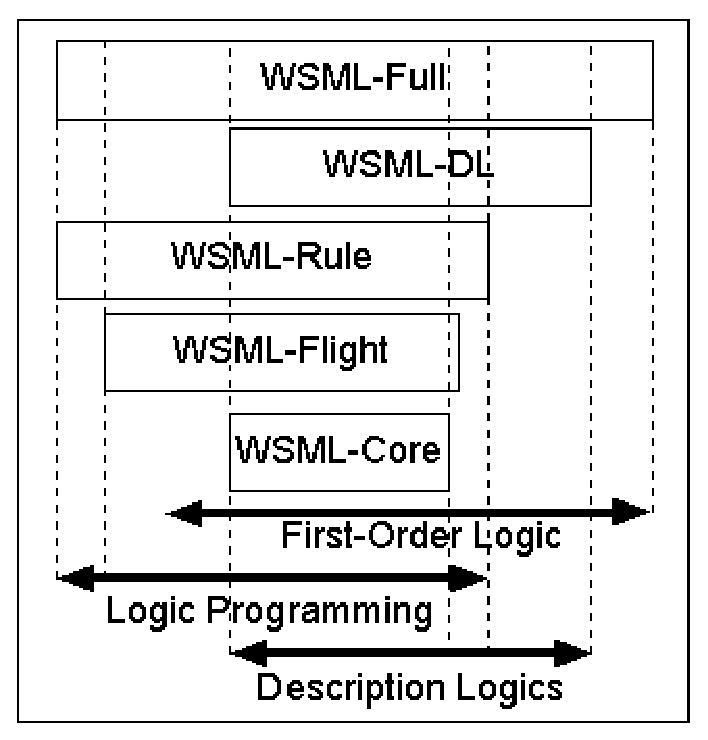
\includegraphics[width=6cm]{images/wsml-layering}
% \caption{Capas de WSML.}
% \label{fig:wsml-layering}
% \end{figure}


 
                                                           
\subsection{Ontolog\'ias}\label{ontologias}
\subsubsection{Antecedentes y Definición}
El desarrollo de las ontologías se deriva directamente de la filosofía, 
Aristóteles acuña el término ``Categoría'' como palabra para describir las
diferentes clases en las que se dividían las cosas del mundo. 
El término ``ontología'' es relativamente moderno (siglo XIX), proviene del griego
$Ontos$ (Ser) y $Logos$ (Palabra), se empezó a utilizar para diferenciar el
estudio de la Teoría de Categorías que se hacía en biología, de hecho, el trabajo de categorización surge en muchas áreas de la
ciencia (filosofía, biología, medicina, lingüística, etc.).

El cuerpo de un esquema de conocimiento, \textit{lo} que se puede representar, está basado en una
conceptualización: objetos, conceptos y otras entidades, que se asume existen en
un determinado dominio y que mantienen unas relaciones entre sí. 

\begin{Frame}
\textit{Una ontología es una especificación (explícita) de una conceptualización}~\cite{GruberOnto}. 
\end{Frame}

Las ontologías, por consiguiente, son sistemas basados en el conocimiento (\textit{\gls{SBC}}) que
sirven como modelo unificado en la representación del mismo, adquiriendo incluso
grado de ingeniería~\cite{isbn1846283965,Benjamins98ontological}. En muchos
casos, la Web Semántica y por extensión las ontologías se apoyan en la
reutilización de conocimiento compartido. Las definiciones realizadas para las ontologías son variadas y todas dejan claro
que sirven para modelar cierto dominio (conjunto de conceptos y relaciones):

\begin{itemize}
  \item Una ontología define los términos básicos y las relaciones establecidas en cierta área.
  \item Especificación explícita de una conceptualización.
  \item Especificación formal y explícita de una conceptualización compartida.
  \item Teoría lógica que provee de forma explícita y parcialmente una conceptualización.
  \item \ldots
\end{itemize}

En el artículo~\cite{Studer98knowledge} los autores agregan
expresividad realizando la siguiente descripción completa de ontología:
\begin{itemize}
  \item Conceptualización, modelo abstracto de algún fenómeno del mundo,
  proveniente de la identificación de los conceptos relevantes de dicho
  fenómeno. \item Explícita, conceptos y restricciones usados se definen
  explícitamente. \item Formal, capacidad de ser legible e interpretable por las
  máquinas.
  \item Compartida, captura conocimiento consensuado.
\end{itemize}

Es posible fusionar las definiciones anteriores en nueva descripción del término ontología:
\begin{definition}
Modelo conceptual organizado mediante una taxonomía que permite definir
relaciones entre conceptos, funciones, instancias (elementos) y axiomas en un determinado
dominio.
\end{definition}

Para completar la definición de ontología hay que tener en cuenta la
nomenclatura que habitualmente se utiliza para nombrar a las distintas entidades
posibles y que en algunos casos puede dar lugar a errores:

\begin{itemize}
  \item Clase, concepto, categoría o tipo.
  \item Instancia, individual.
  \item Entidad, objeto (clase o instancia).
  \item Propiedad, relación, slot, atributo, rol.
\end{itemize}

En la actualidad, la construcción de sistemas basados en conocimiento conlleva la
creación partiendo de cero de nuevas bases de conocimiento. La aspiración debería ser
utilizar componentes reutilizables~\cite{Gruber93towards}, de esta manera los desarrolladores deberían
crear sistemas con la agregación del conocimiento ya existente. El conocimiento definido, 
las técnicas de resolución de problemas y otros servicios, podrían ser
compartidos entre varios sistemas, impulsando la creación de grandes sistemas con
un bajo coste. Desde esta perspectiva, se pueden usar las ontologías como
infraestructura para sistemas ubicuos.

\subsubsection{Componentes}
Una ontología consta de un conjunto no vacío de conceptos identificados como
relevantes en el dominio a modelar, un conjunto de atributos para describir los
conceptos que pueden proveer de distintas fuentes: propios, heredados, etc., un
conjunto de funciones, un conjunto de axiomas que formalizan las condiciones que
deben cumplir los distintos conceptos y un conjunto de instancias o
realizaciones particulares de los conceptos.

\begin{description}
\item[Conceptos:] cualquier entidad que se puede describir, tiene asociado un
identificador único, puede poseer diferentes atributos y establecer relaciones
con otros conceptos.
\item[Relaciones:] representan la interacción entre los conceptos de dominio.
Formalmente, se definen como subconjuntos del producto cartesiano de $n$
conjuntos $R: C_1 \times C_2 \times \ldots \times C_n$.

No todas las relaciones tienen el mismo significado, existen relaciones binarias
de especialización como (\textit{is-a}) o de composición (\textit{part-whole}),
que se modelan con las propiedades clásicas simétricas, reflexivas, etc.

\item[Funciones:]relaciones en las cuales el elemento \textit{n-ésimo} es único para
los $n-1$ anteriores. Formalmente, se definen como $F:C_1 \times C_2 \times
\ldots \times C_n$. Por ejemplo una relación \textit{serPadreDe} se puede
modelar como una función ya que el atributo que evalúa es único para cada caso.

\item[Axiomas:] modelan ``verdades'' que siempre se cumplen en el modelo.
Existen dos tipos de axiomas:
\begin{itemize}
  \item Estructurales, condiciones relacionadas con la estructura jerárquica de
  la ontología. 
  \item No estructurales, establecen relaciones entre atributos de un concepto y
  son específicos de cada dominio.
\end{itemize}

\item[Instancias:] representan realizaciones específicas del dominio de la ontología.
\end{description}

\subsubsection{$Description Logics$ y ontologías}
\textit{Description Logics}~\cite{baader03description} (\gls{DL}s) son un conjunto de lógicas
formales en el área de \textit{Knowledge Representation}, utilizadas para la representación y
razonamiento del conocimiento en un dominio de forma no ambigua. Las DLs se
basan en una semántica perfectamente definida que provee un conjunto de
constructores y primitivas con un significado lógico preciso.

Los pilares de estas lógicas son dos conjuntos: uno de ellos, \textit{atomic concepts}
o predicados unarios y otro, \textit{atomic roles} o predicados binarios. Una
DL provee además un conjunto de operadores, llamados \textit{constructores}, que
permiten crear conceptos y roles más complejos a partir de los más sencillos.
Tanto los conceptos atómicos como los complejos, se denominan uniformemente \textit{conceptos}
y de igual forma, los roles atómicos y los complejos se denominan
\textit{roles}.

Los conceptos se utilizan para representar conjuntos de objetos y los roles
sirven para establecer relaciones binarias entre objetos. Podemos definir el
conjunto de los números reales como la disyunción de
números racionales e irracionales
\begin{example}
$ \mathbb{R} \equiv \mathbb{Q} \sqcup \mathbb{I}$
\end{example}

En general, una base de conocimiento basada en DL consiste en:
\begin{itemize}
  \item \textit{TBox}, contiene los axiomas de inclusión de conceptos
  $C_1 \sqsubseteq C_2$.
  \item \textit{RBox}, contiene los axiomas de inclusión de roles $R_1 
  \sqsubseteq R_2$.
  \item \textit{Abox}, contiene axiomas (aserciones sobre conceptos) $C(a)$, las
  aserciones sobre los roles $R(a,b)$, $a$ y $b$ son son nombre de objetos, $R$
  es un rol y $C$ es un concepto.
\end{itemize}
 
Los constructores booleanos de conceptos son la $\sqcup$ (disyunción o unión),
$\sqcap$ (conjunción o intersección) y $\neg$ (negación). Una
DL que provee, implícita o explícitamente, todos los operadores booleanos se
considera \textit{cerrada} (proposicionalmente). Las DLs ``cerradas'' serán las
que sean interesantes para su procesamiento en la Web Semántica. Aparte de los
operadores booleanos, habitualmente las DLs proveen otros constructores para
generar conceptos complejos a partir de roles. En este apartado, se encuentran
los operadores existencial ($\exists$)  y universal $\forall$. 

Las DLs que proveen estos cinco operadores se denominan $\mathcal{ALC}$, pero
esta lógica no permite axiomas de inclusión en roles y la componente 
\textit{RBox} es vacía, supone que si bien se pueden realizar operaciones
de razonamiento, la lógica a este nivel es poco expresiva. Añadiendo nuevos
constructores a $\mathcal{ALC}$ se obtiene el conjunto de lógicas
$\mathcal{ALC_{HR^+}}$ (también conocida como $\mathcal{SH}$), que resultan de añadir la
inclusión de axiomas (permitiendo diferentes tipos), sobre la \textit{RBox}.
Esta familia de lógicas, ver Tabla ~\ref{table:sh} extraída de~\cite{Cuenca}, es muy
interesante porque posee un gran poder expresivo y puede ser probada sobre razonadores DL, como FaCT++, Racer, Pellet o Hermit.


\begin{table}[htb]
\renewcommand{\arraystretch}{1.3}
\begin{center}
\begin{tabular}{|c|c|c|}
\hline
\textbf{Nombre constructor}&\textbf{Sintaxis}&\textbf{Lógica}\\
\hline
Concepto atómico& $A$ & \\
Concepto universal& $(\top)$ & \\
Rol atómico& $R$ & \\
Conjunción de conceptos& $C \sqcap D$ & \\
Disyunción de conceptos& $C \sqcup D$ & \\
Negación de concepto& $\neg C$ & \\
Restricción existencial& $\exists R.C$ & \\
Restricción universal& $\forall R.C$ & \\
Rol transitivo& $Trans(R)$ & $\mathcal{S}$\\
\hline
Jerarquía de roles& $R_1 \sqsubseteq R_2$ & $\mathcal{H}$\\
\hline
Inversión de roles& $(R^-)$ & $\mathcal{I}$\\
\hline
Nominales (instancias)& $\{o\}$ & $\mathcal{O}$\\
\hline
Restricciones funcionales de número& $\geq 2S  (\geq 1S)$ &
$\mathcal{F}$\\ \hline

Restricciones no cualificadas de número& $\geq nS  (\leq nS)$ &
$\mathcal{N}$\\ 

\hline

Restricciones cualificadas de número& $\geq nS.C  (\leq nS.C)$ &
$\mathcal{Q}$\\ 

\hline
\hline

\end{tabular}
\caption{Familia de lógicas $\mathcal{SH}$.}
\label{table:sh}
\end{center}
\end{table}

La lógica DL es importante para la construcción de ontologías ya que permite
construir bases de conocimiento formales, computables y no ambiguas. Aunque no siempre será indispensable este nivel 
de lógica, tanto para la descripción de dominios como para la Web Semántica, es necesario presentar y dar a conocer este conjunto
de lógicas, para así validar los modelos y mantener unos criterios
formales en la construcción de ontologías. Las ontologías construidas con lógica
DL proporcionan una base sólida para el desafío de la Web Semántica.


\subsubsection{Ontología como \textit{SBC}}
Como sistema basado en el conocimiento, ver Figura~\ref{fig:knowledge}, y teniendo en
cuenta la importancia de la utilización de \textit{Description Logics} como lógica para
la creación de ontologías, se pueden distinguir los tres componentes heredados de
la definición de \gls{DL}. Pero desde el punto de vista tanto del razonamiento como la
inferencia, operaciones importantes en cualquier \gls{SBC}, resultan de interés los
siguientes componentes: 1) \textit{Tbox}, parte terminológica (organizado jerárquicamente) o
conocimiento definido por intensión, consistente en conceptos, roles y construcciones más complejas por combinación de éstos y 
2) \textit{Abox} o parte extensional, es decir,  las afirmaciones sobre individuos``concretos''. Sobre estas dos componentes se podrá realizar
razonamiento, operación especialmente relevante para la Web Semántica, de dos formas:

\begin{description}
\item[Razonamiento \textit{Tbox}, intensional o estructural:] permite consultar la estructura de
conocimiento e inferir información a partir de ella. El mecanismo de
razonamiento estructural por excelencia es la subsunción de conceptos, permite
calcular todos los subconceptos a partir de un concepto dado o consultar si un concepto
es subconcepto de otro. Los razonamientos usuales en la \textit{Tbox} son: \begin{itemize} \item Consistencia, comprueba si el conocimiento tiene o no sentido. 
\item Subsunción, comprobación de sí todos los individuos que pertenecen a un concepto (el
subsumido) también pertenecen a otro concepto (el que subsume). \item 
Equivalencia, comprueba si dos clases denotan el mismo conjunto de instancias. \end{itemize}

Todos estos razonamientos son aplicables al problema de la satisfacibilidad de
fórmulas lógicas siempre que se utilice un lenguaje de definición de conceptos que
sea cerrado con respecto a la negación.

\item[Razonamiento \textit{Abox} o extensional:] permite inferir nuevas instancias a partir de las
definidas de forma explícita en la \textit{Abox}. Los razonamientos usuales en la \textit{Abox} son:
\begin{itemize}
\item Comprobación de instancias, verifica que un determinado individuo es una instancia de un concepto específico. 
\item  Consistencia de la base de conocimiento, implica verificar que cada
concepto que existe en la base de conocimiento admite, al menos, una instancia o
individuo. 
\item Realización, encuentra el concepto más
especifico del que un individuo es instancia.\end{itemize}

\end{description}

\begin{figure}[htb]
\centering
	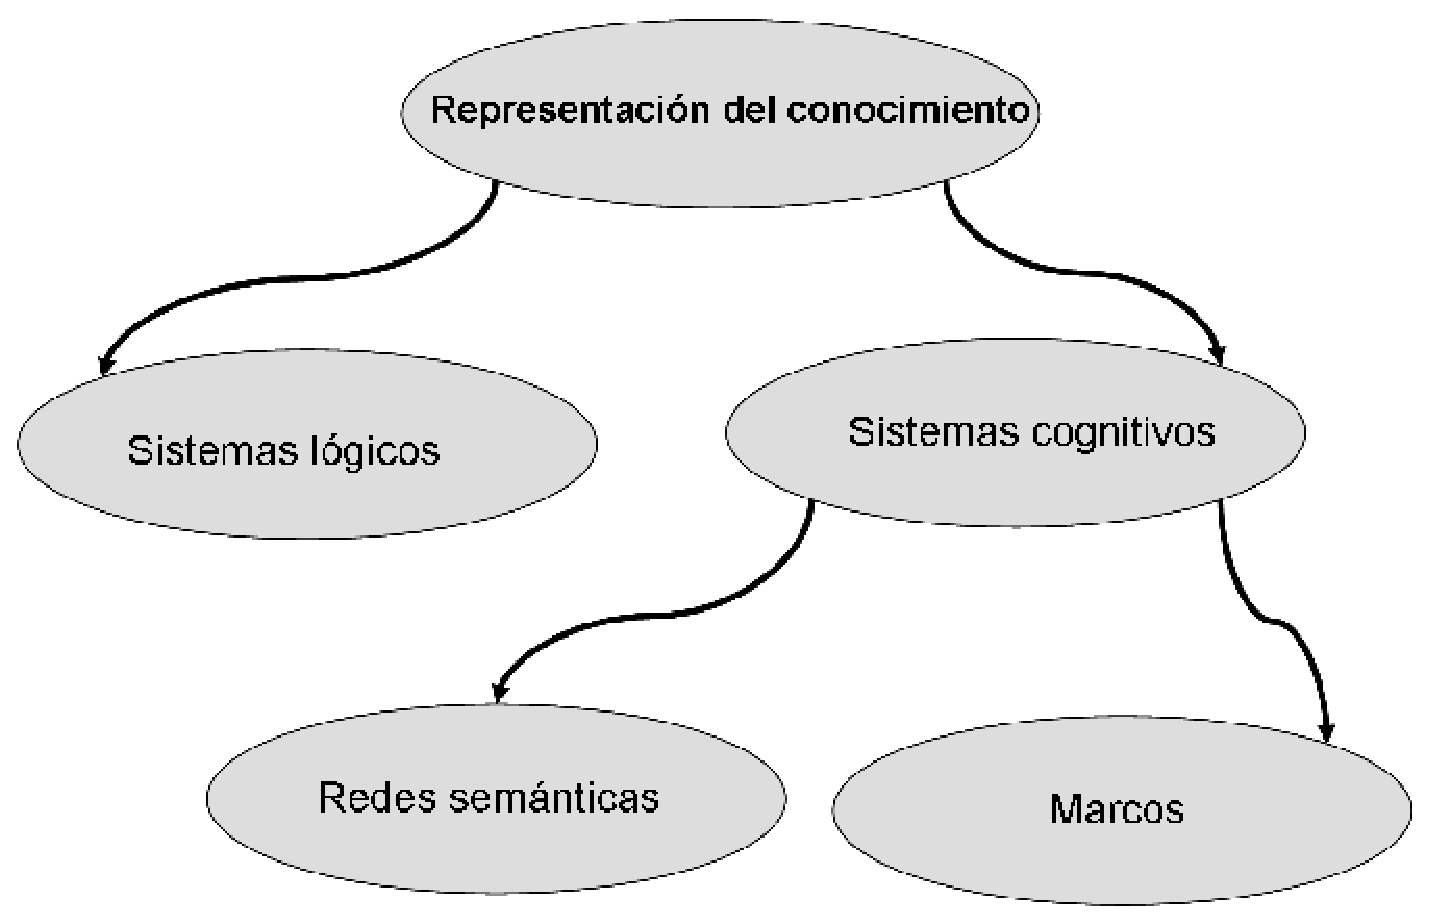
\includegraphics[width=10cm]{images/knowledge}
\caption{Sistemas basados en conocimiento.}
\label{fig:knowledge}
\end{figure}


\subsubsection{Clasificación de ontologías}
Las ontologías se pueden clasificar atendiendo a diferentes a criterios, a
continuación se exponen algunos de ellos.
\begin{description}
 \item [Grado de axiomatización.] Atendiendo a Sowa~\cite{Sowa99knowledge} las ontologías se pueden clasificar en:
\begin{description}
\item[Terminológicas:] define términos y sus relaciones en taxonomías que
involucran tanto relaciones de subtipo y supertipo, como las que relaciona
partes con un todo (\textit{part-whole}), no incluyen axiomas y definiciones
expresadas en lógica o lenguaje formal interpretable por una máquina. Por lo
tanto, existe menos información sobre el dominio modelado pero la simplicidad de
su especificación permite construir ontologías de gran tamaño.
\begin{example}
WordNet base de conocimiento (y datos) léxica.


Fuente: \url{http://wordnet.princeton.edu/}
\end{example}

\item[Formales:] consta de categorías restringidas por axiomas y definiciones
expresadas en alguna lógica formal, con menos conceptos pero preparadas para soportar
un procesamiento automático y servicios de razonamiento.

Una ontología terminológica podrá convertirse en formal a medida que se añadan
axiomas, aunque esta evolución no es ni mucho menos trivial.
\end{description}

\item[Según contexto.] Dependiendo del grado de dependencia del contexto las ontologías pueden ser:
\begin{description}
\item[Dominio:] modelan conceptualizaciones específicas, con restricciones de
estructura y contenido del dominio. Se reaprovecharán sólo en aquellas
aplicaciones que trabajen en ese dominio. Grado de dependencia alto.

\begin{example}
Ontología de medicina \textit{Galen}.


Fuente: \url{http://www.opengalen.org/}.
\end{example}

\item[Generales o de sentido común:] vocabularios o estructuras taxonómicas
genéricas. Alto grado de reaprovechamiento y bajo de dependencia del dominio.

\begin{example}
Cyc y OpenCyc.


Fuente: \url{http://www.cyc.com/}. 
\end{example}

\item[Metaontologías u ontologías genéricas:] ontologías de dominio genérico,
conceptos universales.
\begin{example}
DOLCE: Descriptive Ontology for Linguistic and Cognitive Engineering.


Fuente: \url{http://www.loa-cnr.it/DOLCE.html}. 
\end{example}

\end{description}

\item [Objeto de creación.]

Atendiendo al objetivo de creación de una ontología se establecen diferentes tipos:

\begin{itemize}
  \item Ontologías para la representación de conocimiento, como: \gls{OWL},
  \gls{DAML+OIL}, \gls{RDF}, RDF(S), OKBC, etc.
  \item Ontologías \textit{top level}, definen \textit{frameworks}, conceptos
  universales como las ya comentadas \textit{DOLCE} o \textit{Cyc}. 
  \item Ontologías para la definición de términos lingüisticos como
  \textit{WordNet} o \textit{EuroWordNet}~\cite{EuroWordNet}. 

	\item Ontologías de dominio, modelan conocimiento de cierto dominio: comercio
	electrónico o \textit{e-commerce}, de medicina \textit{Galen} o SNOMED, etc. 
\end{itemize}

\end{description}

Las ontologías como sistemas basados en conocimiento, serán más productivos
cuanto mejor ``informados'' estén, por ello, será interesante modelar utilizando
el mayor de grado de particularidad posible en el dominio, pero teniendo presente, que también es
importante mantener el objetivo de reutilizar conocimiento, podría ser interesante
enclavar los nuevos conceptos de dominio definidos dentro de las categorías de
alto nivel, para así alinear estas definiciones en un marco conceptual genérico.


\subsubsection{Principios de diseño}\label{onto-design}
Las ontologías deben o deberían cumplir una serie de principios:
\begin{description}
\item[Claridad:] proporcionar el significado pretendido a los términos
definidos. Definiciones tan objetivas como sea posible.
\item[Completitud:] las definiciones deberían recoger todas las condiciones
necesarias y suficientes, además de poseer una buena documentación en lenguaje natural.
 \item[Coherencia:] los términos definidos deben ser coherentes, concluyendo
 sólo aquellas inferencias consistentes con el modelo definido.
 \item[Extensibilidad:] anticipando la necesidad de reutilización y facilitando
 la adición de nuevo \linebreak conocimiento.
 \item[Mínimo compromiso ontológico:] minimizar el número de afirmaciones a
 realizar sobre el dominio modelado, permitiendo así que otros agentes las
 puedan refinar.

\item[Diversificación de jerarquías:] haciendo uso de la herencia múltiple, usar
tantos criterios de clasificación como sea posible. Así, añadir un nuevo concepto
es sencillo utilizando los ya existentes y la capacidad de clasificación.

\item[Minimizar la distancia semántica entre hermanos:] conceptos similares
deben agruparse.
 
  \item[Estandarización:] independencia simbólica, utilización de nombrado estándar.
 \item[Granularidad:] coherencia en el grado de particularidad, evitando el uso
 de términos ambig\"{u}os.
\end{description}

Finalmente, existen diversos procesos de desarrollo o metodologías que definen un
procedimiento para la captura de conocimiento de un dominio y la pertinente
construcción de ontologías. Por ejemplo: \textit{Methontology Framework} o \textit{Sensus method}. 


\subsubsection{Operaciones con ontologías}\label{op-ontologias}
En esta sección se describen las
operaciones~\cite{bruijn06-seman-web} que se pueden
realizar con las ontologías de acuerdo a su principio de reaprovechar el
conocimiento ya definido. La reutilización del conocimiento consensuado  es una de las
máximas de la creación de ontologías, para ello se definen tres operaciones
básicas (\textit{mapping} o correspondencia entre ontologías, \textit{merging} o
unión de ontologías y \textit{alignment} o descubrimiento de las
correspondencias de \textit{mapping} ) que
ayudan a la agregación de conocimiento basado en ontologías. La
importancia de estas operaciones se pone de manifiesto en la mediación de datos
entre fuentes heterogéneas, aspirando a resolver los conflictos que se producen
entre sistemas basados en conocimiento, que deben interaccionar entre sí pero que
han sido creados independientemente. El proceso de mediación, adquiere especial
interés para la propuesta de servicios web semánticos, en los cuales esta
operación es básica debido a la integración de ontologías provenientes de
diferentes modelos de negocio.  


\begin{description}
\item[\textit{Mapping} o \textit{mapeo} de ontologías:] especificación declarativa del
solapamiento semántico entre dos ontologías. Las correspondencias entre
entidades de ontologías diferentes son expresadas mediante axiomas en un
determinado lenguaje de \textit{mapeo}. Este proceso consta de tres fases: descubrimiento, representación y ejecución. Existen diferentes enfoques para llevar a cabo esta operación
como MAFRA, RDFT o C-OWL.
\item[\textit{Alignment} o alineamiento de ontologías:] proceso mediante el cual
se descubren las similitudes entre dos ontologías. El resultado es una especificación de los puntos en común, realizada a través del algoritmo 
\textit{Match operator}. Existen diferentes implementaciones como
Anchor-PROMPT, \linebreak GLUE, \textit{Semantic Matching} o QOM.
\item[\textit{Merging} o unión de ontologías:] creación de una ontología nueva
tomando como fuente dos o más ontologías. La nueva ontología unifica y reemplaza
las ontologías fuente. Se establecen dos enfoques para realizar esta
operación: 1) entrada de $n$ ontologías y salida de una sola
ontología, unión y reemplazo de las demás (por ejemplo: algoritmo
PROMPT~\cite{NM00}) y 2) entrada $n$ ontologías que no son reemplazadas, sino que se genera una ontología
\textit{bridge} que importa a las ontologías originales y especifica las correspondencias mediante
axiomas \textit{bridge}, por ejemplo \textit{OntoMerge}.
\end{description}

A la hora de afrontar la implementación de estas operaciones sobre ontologías se pueden generar dos tipos básicos de conflictos que impiden el éxito de la
operación y requieren intervención humana para facilitar la realización
automática de las operaciones: 
\begin{enumerate}
  \item Conflictos entre ``conceptualizaciones'' distintas del mismo dominio. A
  su vez, se distinguen dos categorías: 1) conflicto de ámbito, ocurre cuando dos clases tienen solapamiento en sus extensiones (el
  conjunto $s$ de instancias), y no coincide exactamente y 2) conflicto en la
  cobertura del modelo y su granularidad, ocurre si dos ontologías cubren parte
  de cierto dominio (por ejemplo: empleados de universidad y estudiantes) o bien
si una es más específica que otra (por ejemplo: una ontología define ``persona'' y otra define ``persona joven'').
  \item Conflictos entre las especificaciones de los conceptos. También, se diferencian tres categorías:\linebreak 1) conflicto en el estilo de
  modelado, cada ontología específica los conceptos de una manera determinada
(por ejemplo: tratamiento de las unidades de tiempo) o la descripción de los
conceptos   difiere (por ejemplo: utilización de subclases vs atributos); 2) conflicto
en la  terminología, dos conceptos son equivalentes pero no utilizan el mismo nombre,
  problema de sinónimos, o viceversa, son diferentes y utilizan el mismo nombre,
  homónimos y 3) conflicto de codificación, no se utilizan las mismas
  nomenclaturas, unidades de medida, etc.
\end{enumerate}

Todos estos conflictos, vienen en muchos casos provocados por no ajustarse a los
principios de diseño establecidos en la Sección~\ref{onto-design}. No
obstante, es habitual afrontar los problemas surgidos en la integración de ontologías ya que los
modeladores provienen de distintas partes, con diferente formación y puede que
sigan procedimientos particulares para la realización del modelado de
las ontologías, facilitando las tareas a las aplicaciones que las consuman.


\subsubsection{Aplicación de las ontologías}
Las ontologías se convierten en la pieza fundamental de ciertas áreas así pueden señalarse las 
siguientes:

\begin{description}
\item[Ingeniería del conocimiento:] las ontologías se pueden manifestar durante la ejecución de las siguientes tareas:
\begin{itemize}
  \item Construcción del modelo conceptual, generando los términos del glosario
  y de las relaciones que se establecen entre ellos.
  \item Construcción de la base de conocimiento, utilizando la ontología de
  modelado conceptual se pueden crear bases de conocimiento con la aplicación de
  reglas, restricciones, etc.
\end{itemize}

\item[Procesamiento del lenguaje natural:] mantenimiento de la definición de términos
gramaticales del lenguaje y las relaciones entre ellos.

\item[Integración de sistemas heterogéneos:] gestión de las diferencias
existentes entre diversos sistemas de información con el objetivo de facilitar
la comunicación entre los mismos.
\item[Búsqueda semántica:] utilizando conceptos y no términos para realizar las
búsquedas. 

\item[Web Semántica:] las ontologías son la base de la Web Semántica, por ello
cualquier aplicación que tenga un carácter semántico se apoyará, muy
probablemente, en ontologías.
\end{description}


Las ontologías se abren paso con fuerza sobre todo en el ámbito de las
aplicaciones~\cite{DBLP:conf/nldb/Penalver-MartinezVS11} de la Web Semántica, en particular en el escenario de la
integración de aplicaciones (servicios web semánticos~\cite{DBLP:journals/es/SanchezSMAVG11}) y contextualización del
usuario. En la construcción de una ontología, hay que afrontar el modelado desde el
punto de vista de la lógica (tipo y lenguaje de expresión) siguiendo los
principios de diseño, ver Sección~\ref{onto-design}, y no de la orientación a objetos, muy frecuente en el ámbito de la ingeniería del \textit{software}.  
   
\chapter{\label{capitulo:semantica}Panorámica de uso de la\\ Linked Data y Open Data} 
\input{chapters/linked-data/linked-data}
\chapter{\label{capitulo:eproc-sm}Tendencias actuales en Semántica} 
El creciente uso de Internet durante los últimos años ha puesto de manifiesto un
nuevo entorno de ejecución para las aplicaciones, utilizando como nueva
plataforma la web, el gran sistema distribuido. Nuevas tecnologías y paradigmas
están emergiendo para dar soporte al desarrollo y despliegue de aplicaciones y
servicios, así como para la publicación de datos e información. Los modelos de
desarrollo están cambiando a un estilo más colaborativo en el cual las empresas
ofrecen su software como servicios (\textit{Software as a Service}-\gls{SaaS}) materializado a
través del paradigma de \textit{cloud computing}~\cite{Armbrust09abovethe}, implementado con tecnología de
servicios con el objetivo de que terceros puedan utilizar estos servicios para
la construcción de aplicaciones agregadas con valor añadido. 

En este sentido, tal como se ha señalado, iniciativas como la Web Semántica que a través de modelos y
formatos de datos de conocimiento compartido unificados, intentan elevar el
significado de los elementos y recursos que están disponibles en la web, con el
objetivo de mejorar la integración e interoperabilidad entre aplicaciones, 
impulsando la implantación de este enfoque. Dentro de la iniciativa de Web
Semántica hay que destacar dos esfuerzos: 
\begin{enumerate}
 \item La iniciativa \linkeddata que como se ha descrito propone la publicación de datos
enlazados siguiendo el modelo \gls{RDF} para facilitar la creación de una web de
datos en la que éstos se puedan mostrar, intercambiar y conectar a través de
URIs. La tendencia actual de publicación de datos enlazados está marcando una
evolución en la interoperabilidad de aplicaciones, con el consiguiente efecto que
conlleva para las relaciones \gls{B2B}, \gls{B2C} o \gls{A2A}. Entre los casos de éxito
podríamos destacar: administración electrónica (iniciativa de \textit{Open Government
Data}, contratación pública de bienes y servicios (\eproc), oferta formacional , contextualización de aplicaciones, \textit{mashups},
etc. 

\item El desarrollo de lenguajes y formalismos lógicos para representar el conocimiento sobre un universo de discurso, permitiendo la inferencia de nuevos
datos a partir de los datos ya publicados. En este contexto se han impulsado nuevamente el uso de las técnicas de razonamiento y de sistemas basados en conocimiento, 
como pueden ser las ontologías y los sistemas basados en reglas (Ontobroker, XSB, etc.) o de producción (Drools , JRules , etc.). 
La aplicación de estos sistemas está ampliamente asentada en la resolución de diversos problemas
(diagnóstico, planificación, reglas de negocio, etc.) pero siempre utilizando un enfoque para la representación del conocimiento y de los datos, en muchos casos
específico y no estandarizado. Por tanto, debe tenerse en cuenta la flexibilidad, tanto para la integración como para la interoperabilidad de las aplicaciones. Una arquitectura orientada a
servicios sobre la plataforma web, utilizando los protocolos actuales y que se beneficie de las iniciativas relativas a la Web Semántica puede dar respuesta a
este punto clave. La implantación de un sistema basado en conocimiento, más en concreto de
sistemas basados en reglas y de razonamiento, que hagan uso de una infraestructura estandarizada y cooperativa puede ser de gran beneficio para la
resolución de problemas basados en conocimiento declarativo y compartido, mejorando tanto la independencia tecnológica de las aplicaciones como la experiencia de usuario.
\end{enumerate}


Al amparo de la visión de la Web Semántica, el \gls{W3C} ha promovido la creación de varias recomendaciones que intentan ofrecer soluciones 
para las diferentes capas de la arquitectura. En concreto, RDF es el lenguaje de representación básico que 
permite representar tripletas de la forma sujeto-predicado-objeto. Dichas tripletas 
forman un grafo dirigido que puede integrarse automáticamente con otros grafos obtenidos de otros servidores. 
Otra de las tecnologías propuestas por el W3C es RDFS, que permite la definición de clases, propiedades e individuos y 
ofrece unos mecanismos básicos de inferencia mediante reglas. RDFS facilita la creación e integración de vocabularios 
pero carece de expresividad suficiente para describir relaciones avanzadas como complementos de conjuntos o cardinalidades. Las limitaciones 
expresivas de RDFS propiciaron la definición de \gls{OWL}, un lenguaje de definición de ontologías basado en lógica descriptiva. 
La versión 2 de OWL llegó a status de recomendación del W3C en octubre del año 2009. Una de las principales mejoras de esta versión era 
intentar resolver el compromiso entre la expresividad y la complejidad de los razonamientos mediante la definición de perfiles o 
fragmentos computacionales. Los tres perfiles de OWL2, EL, QL y RL son sublenguajes del mismo que permiten alcanzar una complejidad 
polinómica para tareas de razonamiento estándar limitando la expresividad. La combinación de OWL con lenguajes basados en 
reglas que incluyen la negación, como los \textit{dl-programs}~\cite{DBLP:conf/rr/Motik08} han sido desarrollados en las redes de excelencia 
\textit{REWERSE} y \textit{Knowledge web} y definen la interoperabilidad entre las reglas y las ontologías. 

El problema del intercambio de reglas entre los distintos sistemas de razonamiento e inferencia también ha sido abordado recientemente, 
así encontramos la recomendación del W3C RIF de 22 de junio del año 2010. 
\gls{RIF} es, de nuevo, una familia de lenguajes (\textit{Core},\textit{Production Rule Dialect, BLD Basic Logic Dialect, Datatypes and Built-Ins, Framework for Logic Dialects}, etc.) 
con diferente expresividad, cuyo objetivo es convertirse en \textit{lingua franca} para el intercambio de conocimiento basado en reglas en la web. 
El formato utilizado por RIF es \gls{XML} y su combinación con ontologías permite que las reglas y el modelo de datos sobre los que se van a aplicar 
las reglas se pueden intercambiar entre distintos actores. Para interpretar RIF es necesario realizar una traducción desde este vocabulario al motor de inferencia
deseado. En el ámbito de intercambio de reglas hay que resaltar el antecesor de RIF, RuleML que es una iniciativa internacional sin ánimo de lucro, que cubre
los aspectos del intercambio y la interoperabilidad de reglas. Esta iniciativa mantiene una estrecha relación con los grupos de OASIS en reglas, así como con
ISO Common Logic (estándar en el año 2007). RuleML, como grupo, también contribuye en \gls{OMG} a \gls{SBVR}, específicamente en el apartado de \textit{Production Rule Representation} (PRR) cuya última
versión data de diciembre del año 2009.

Para la consulta de datos \gls{RDF} se ha desarrollado \gls{SPARQL}, un lenguaje de consulta y un
protocolo de acceso que permiten definir un terminal (o \textit{endpoint}) en el que se publican conjuntos de datos (o datasets) RDF y que pueden accederse
como servicios en la web. Actualmente se está trabajando en vocabularios para
definir datasets y poder enlazarlos entre sí de forma sencilla. Con el uso de
SPARQL han aparecido propuestas para la definición de reglas de producción con
este lenguaje (extensión \textit{SPARQL with Updates-\gls{SPARUL})} de modo que se ejecuten
directamente sobre una base de datos en RDF, como puede ser SPARQL-Rules~\cite{citeulike:1294570},
también existen enfoques para la consulta de ontologías OWL con SPARQL~\cite{Sirin07sparql-dl:sparql} y
en la especificación en la que se está trabajando al presente, SPARQL 1.1, se
dispone de un vocabulario para definir los servicios disponibles. Finalmente y
con el objetivo de personalizar la vista de las aplicaciones por el usuario y su
contextualización se ha aplicado el uso de reglas en formato \gls{JSON}~\cite{conf/ki/GiurcaP08}. 


La evolución de los formalismos para definir ontologías lleva emparejado el
desarrollo de razonadores que puedan llevar a cabo las inferencias necesarias.
Desde el pionero KL-ONE hasta este momento, se han implementado múltiples
razonadores basados en lógica descriptiva siguiendo diferentes técnicas. En la
actualidad, se pueden destacar Fact++~\cite{Tsarkov2006}, Pellet~\cite{Sirin_Parsia_Grau_Kalyanpur_Katz_2007} y RacerPro~\cite{Rajeev2001Racer}
que se basan en la técnica conocida como \textit{semantic tableaux}. A pesar de las altas
complejidades, en el caso peor los algoritmos de razonamiento utilizados en estos sistemas son capaces de resolver muchas tareas prácticas gracias al uso de
diversas optimizaciones. Para resolver dichas limitaciones, especialmente, al
tratar con grandes cantidades de datos, se han buscado técnicas alternativas
como el algoritmo de resolución utilizado en KAON2~\cite{journals/ercim/Motik08}, el sistema
\textit{hipertableau} empleado en HermiT~\cite{msh09hypertableau}, las técnicas de eliminación de tipos~\cite{DBLP:conf/aaai/RudolphKH08}
 o las recientes técnicas basadas en eliminación de consecuentes~\cite{DBLP:conf/ijcai/SimancikKH11}.

La utilización de reglas se ha propuesto como una alternativa para la
implementación de razonadores. En este caso, las definiciones de la ontología
son compiladas a un conjunto de reglas, que se aplica al conjunto de datos para obtener las inferencias correspondientes. La principal
ventaja de estos razonadores es que se basan en técnicas ya conocidas en el
ámbito de la programación lógica con diversas implementaciones disponibles, es sin embargo una
desventaja, que generalmente es necesario utilizar subconjuntos de \gls{OWL}, como el
conocido OWL Horst~\cite{Horst2005}. Uno de los mayores retos de la Web Semántica es la búsqueda de técnicas que
mejoren la escalabilidad de los razonadores, en esta línea, han surgido
trabajos que proponen la utilización de tecnologías distribuidas para afrontar
dicha complejidad. Por ejemplo, en~\cite{SomaPrasanna2008}
se propone la implementación de un sistema de inferencia paralelizable sobre OWL
Horst, mediante un particionado de las reglas. Con el objetivo de mejorar la
escalabilidad, en~\cite{springerlink:10.1007/978-3-642-04930-9_43} se propone un algoritmo para realizar inferencias sobre
RDFS que se aplica a un \textit{benchmark} de $10.000$ tripletas, proponiendo como trabajo futuro la posible aplicación de MapReduce~\cite{citeulike:430834,DBLP:conf/semweb/UrbaniKOH09}. En~\cite{UrbaniMaassenBal2010} se describe una implementación basada en el algoritmo MapReduce
logrando realizar el cierre parcial de $864$ millones de tripletas en RDFS en una
hora utilizando 32 procesadores. Recientemente, los mismos autores
desarrollaron el sistema WebPIE~\cite{Urbani2010WebPIE}, el cual ha sido capaz de
realizar inferencias sobre $1$ billón y medio de tripletas en $6,1$ horas utilizando
$32$ nodos, mediante reglas de OWL Horst. El sistema SAOR se ha implementado para
dar soporte al buscador semántico SWSE, incorporando un razonador sobre OWL
Horst~\cite{HoganHarthPolleres2009}, dicho sistema ha diseñado un nuevo algoritmo
distribuido, mejorando la escalabilidad de la implementación~\cite{DBLP:conf/semweb/HoganPPD10}. Finalmente, también se está 
trabajando~\cite{HausenblasCloudLOD} en la conjunción de \linkeddata y \textit{cloud computing} para el procesamiento de grandes cantidades de datos.


\chapter{\label{capitulo:eproc-sm}\textit{e-Procurement} y Semántica} 
La construcción de un modelo semántico sobre un dominio de negocio concreto
consiste en el desarrollo de un sistema de conocimiento que describa las
entidades y propiedades, así como las relaciones lógicas que existen entre
las mismas. Un aspecto, muchas veces minusvalorado, es que en estos modelos de
dominio es necesario describir también los procesos, las restricciones y en
general, los aspectos dinámicos del dominio. Este tipo de modelos formalizados
mediante un lenguaje lógico, como ya se ha descrito, se denominan ``ontologías''. La selección de la lógica apropiada para la modelización de 
la base de conocimiento no es una cuestión sencilla y se deberán contemplar diferentes
factores tales como grado de computabilidad, decidibilidad, soporte razonadores, etc. Existen
diferentes vocabularios y lenguajes que permiten modelar un cierto dominio, algunos
de los cuales ya se han repasado (\gls{RDF}, RDFS, \gls{OWL} y \gls{WSML}) en la Sección~\ref{sect:arch-ws}, no obstante, existen otros estrechamente
ligados a entornos de negocio, que a continuación se presentan.


\begin{description}
\item[\gls{RIF} (\textit{Rule Interchange Format})~\cite{rif-core}.] RIF constituye una familia de lenguajes con diferente expresividad, 
cuyo objetivo es convertirse en \textit{lingua franca} para el intercambio de
conocimiento basado en reglas en la Web. Define la compatibilidad con
documentos RDF y OWL, además está especialmente diseñado para integrarse con
sistemas de inferencia basados tanto en reglas de producción, como de
Programación Lógica. La ventaja de RIF respecto de OWL es una mayor expresividad, 
que permite expresar conocimiento causal y procedimental. 


\item [\gls{SCOR} Model (\textit{Supply-Chain Operations Reference-Model}).] Es un modelo conceptual de
referencia para la especificación y formalización de los procesos de negocio
asociados a las cadenas de suministro. Este modelo define los procesos de
planificación, fabricación, entrega, evolución e inventarios de productos en una
cadena logística.

\item [\gls{SBVR} (\textit{Semantics of Business Vocabulary and Business Rules}).] Es un estándar
(ISO 704/1087) desarrollado por el \textit{Object Management Group} (\gls{OMG}). Define un
metamodelo para el desarrollo de modelos semánticos de vocabularios y reglas de
negocio. La idea es que a partir del lenguaje natural se puedan expresar
vocabularios y reglas de negocio en un dominio concreto. La construcción de un
modelo de negocio mediante el SBVR recoge el vocabulario de conceptos del
dominio y la definición de lógica formal asociada.

\item [Clasificaciones de productos de comercio electrónico~\cite{Leukel-ecatalog2005,Leukel-standard,Leukel-automating}.] Para
facilitar el intercambio automático de información y la anotación de los diferentes productos
y documentos que forman parte del comercio electrónico, distintos sectores de
actividad económica han desarrollado sus propias terminologías o
vocabularios~\cite{Norbert-class} controlados, para armonizar mediante códigos unívocos la identificación de
los objetos de negocio. Ejemplos de estos vocabularios son: el estándar eCl@ss o
la clasificación \gls{UNSPSC} entre otros, ver Sección~\ref{sect:pscs}.


\item [\gls{ebXML} (\textit{Electronic Business using eXtensible Markup Language}).] Es un lenguaje
\gls{XML} elaborado por \gls{OASIS} y UN/CEFACT, también consta de una infraestructura que permite la comunicación entre entidades
participantes en transacciones de negocio electrónico, favoreciendo la interoperabilidad y la seguridad de una forma homogénea entre las distintas partes.
La propuesta original cubría cinco capas: \textit{Business processes}; \textit{Collaboration protocol agreements};
\textit{Core data components}; \textit{Messaging} y \textit{Registries and repositories}.

eBXML ha sido aprobado por \gls{ISO} en un conjunto de especificaciones, ISO 15000:  ISO 15000-1: ebXML \textit{Collaborative Partner Profile Agreement};
ISO 15000-2: ebXML \textit{Messaging Service Specification}; ISO 15000-3: \textit{ebXML Registry Information Model}; ISO 15000-4: ebXML \textit{Registry Services Specification};
y ISO 15000-5: ebXML \textit{Core Components Technical Specification}, Version 2.01.

\item [\gls{XBRL} (\textit{extensible Business Reporting Language}).] 
Es una norma elaborada en el año 1998 por Charles Hoffman, contable y auditor, para
simplificar la automatización del intercambio de información financiera mediante
el uso del lenguaje XML. La familia de lenguajes XBRL se ha realizado para
satisfacer las exigencias principalmente de información financiera y
empresarial, permite aplicar etiquetas identificativas multilenguaje con
significado, por ejemplo indicando si es un valor monetario, también es posible
mostrar la relación que guardan los elementos entre sí, así se podría saber cómo se
calculan. Una característica muy importante es la capacidad de extensión, de
esta forma es capaz de adaptarse para casos particulares de empresas. 

\end{description}

\subsection{Actividades de aplicación de Semántica en \textit{e-Procurement}}
Desde la creación del movimiento de la Web Semántica, en concreto de la realización
práctica mediante \linkeddata, se han aplicado los principios de estas iniciativas a múltiples
dominios como ya se ha reseñado en las secciones anteriores. Evidentemente en un sector como 
la Administración Pública, caracterizado por su amplitud, casuística y carácter estratégico para todos los ciudadanos
es por lo que la semántica y sobre todo las corrientes de \opendata y \linkeddata han penetrado con mucha fuerza en los últimos años. 
En un principio los esfuerzos como en otros dominios, se centraban en el modelado de la administración
como organización y de sus procesos, con el objetivo de mejorar la interoperabilidad e integración
entre las aplicaciones y facilitar los trámites burocráticos. En muchos casos se han desplegado
soluciones flexibles basadas en la reutilización de información, procesos y conocimiento a través
de grandes bases de datos compartidas, servicios web y sistemas basados en reglas, no obstante la inmersión
de la semántica propiamente dicha se centraba en la realización de modelos para formalizar
cuestiones relativas a documentación y a procesos administrativos. Por ello,
la irrupción de \opendata y \linkeddata ha reorientado el esfuerzo de las Administraciones Públicas
para aprovechar la semántica en su beneficio. 

Por otra parte, también han surgido iniciativas~\cite{DBLP:journals/tcci/Alor-HernandezAJPRMBG10} relacionadas con \eproc, pero desde un punto de vista
de las cadenas de suministro, en las cuales se modelan de forma completa un entorno de proveedores y suministros mediante la coordinación
de los recursos software, hardware y humanos propios de un entorno de este tipo, como son \gls{ERP}s, robots o las propias personas. 

\subsubsection{Ontología de Contratos Públicos del proyecto LOTED}
El diseño de la ontología en el proyecto LOTED~\cite{loted-project}, es de suma importancia debido a su consideración 
como primer gran esfuerzo por aunar las iniciativas de \linkeddata y \opendata en el campo de la contratación 
pública electrónica. En este proyecto la propuesta principal consiste en la transformación directa 
de la información proveniente del \gls{RSS} de \gls{TED} a \gls{RDF} para su posterior indexado en un repositorio y acceso 
mediante un \textit{endpoint} de \gls{SPARQL}. Como sucede un muchos casos relacionados con la iniciativa 
de \linkeddata la ontología realizada, ver Figura~\ref{fig:public-contracts-ontology-loted}, está orientada a la representación de los datos en sí, estableciendo 
un modelo formal en el cual enclavar los recursos RDF generados, pero si bien este enfoque es válido, tan sólo 
representa una parte de la casuística presente en el dominio de la contratación pública electrónica. El intento 
realizado en TED se centra en el diseño de las entidades presentes en la información del RSS para así suministrar 
un modelo formal a los recursos RDF. Por todo ello, esta ontología sirve como una gran fuente de información 
para comprobar que tipo de entidades se recogen o publican en el RSS de TED, pero en un espectro más amplio 
se considera insuficiente para la representación de información teniendo en cuenta los modelos de datos 
disponibles en las plataformas de contratación o el propio de \gls{opXML} realizado en el proyecto ``10ders Information 
Services'', como ha quedado señalado en la Sección~\ref{data-model-eproc}. 

Por otra lado y desde el punto de vista del acceso a los datos, se ofrece la posibilidad de la realización 
de consultas en SPARQL seleccionando una serie de códigos y acotando los resultados por fechas, sin embargo este sistema 
parece desactualizado y no se han realizado cambios en los últimos dos años. 

\begin{figure}[h]
 \centering
    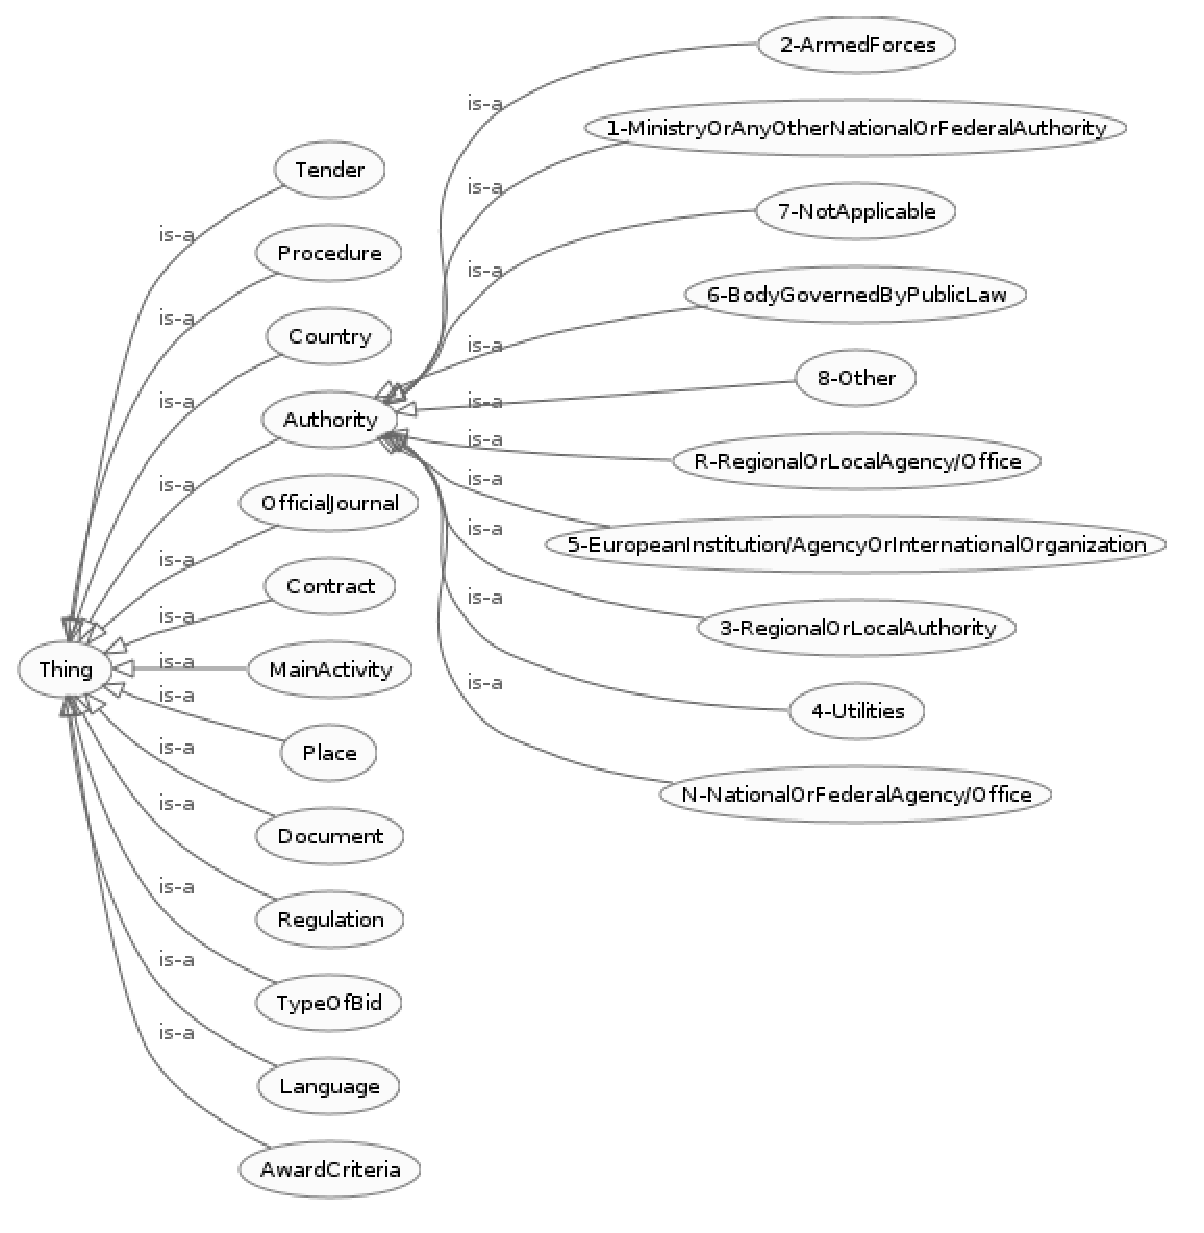
\includegraphics[width=14cm]{images/phd/loted-ontology}
  \caption{Ontología de Contratos Públicos del proyecto LOTED.}
 \label{fig:public-contracts-ontology-loted}
\end{figure}

\subsubsection{Ontología de Contratos Públicos de la República Checa}
Esta ontología está siendo desarrollada por el grupo \textit{Knowledge Engineering Group} 
de la \textit{Charles University} de Praga en la República Checa. Parte del esfuerzo está siendo
cubierto parcialmente dentro del proyecto europeo LOD2 en su paquete de trabajo \textit{WP9A – LOD2 for a Distributed Marketplace for Public Sector Contracts}, cuya descripción es la siguiente:

\begin{Frame}
\textit{The objective of this use case is to explore and demonstrate the application of linked data principles for procuring contracts in the public sector...}
\end{Frame}

Este trabajo enlaza perfectamente con el propósito de este documento, esto es cubrir el sector de los contratos
públicos con semántica y concretamente con la iniciativa \linkeddata. Es por ello que se ha establecido
contacto con los integrantes del grupo de investigación de esta Universidad para aprovechar y realimentar
esfuerzos, como fruto de esta colaboración han empezado a reutilizar los códigos CPV, resultado de este trabajo y del proyecto ``10ders Information Services''.

La ontología que se ha desarrollado en este grupo, ver Figura~\ref{fig:public-contracts-ontology}, tiene como intención recoger
la información y datos de los contratos públicos de forma estructurada, para que pueda ser consumida
automáticamente tanto por personas como por máquinas, desarrollándose también dentro del ámbito
de la iniciativa de \opendata de la República Checa. Desde un punto de vista del diseño reutiliza varios
vocabularios y ontologías ya disponibles, como \textit{Payments Ontology} del Reino Unido, lo que confiere a este modelo un carácter integrador y 
reutilizable. No obstante, abordar la descripción de toda la casuística del proceso de contratación pública electrónica parece
muy ambicioso y podría presentar problemas de interoperabilidad, integración y reutilización ya que 
puede estar muy orientada a la problemática de un entorno particular. Otro de los puntos importantes
que se deben abordar, y parcialmente recogidos en esta ontología y que deben servir de guía, están referidos a 
la adición de metainformación para \textit{provenance}, licencia, etc., que si bien en algunos
\datasets es importante, en la información de carácter público es fundamental y debe ser un requisito
para las propias entidades públicas.

\begin{figure}[h]
 \centering
    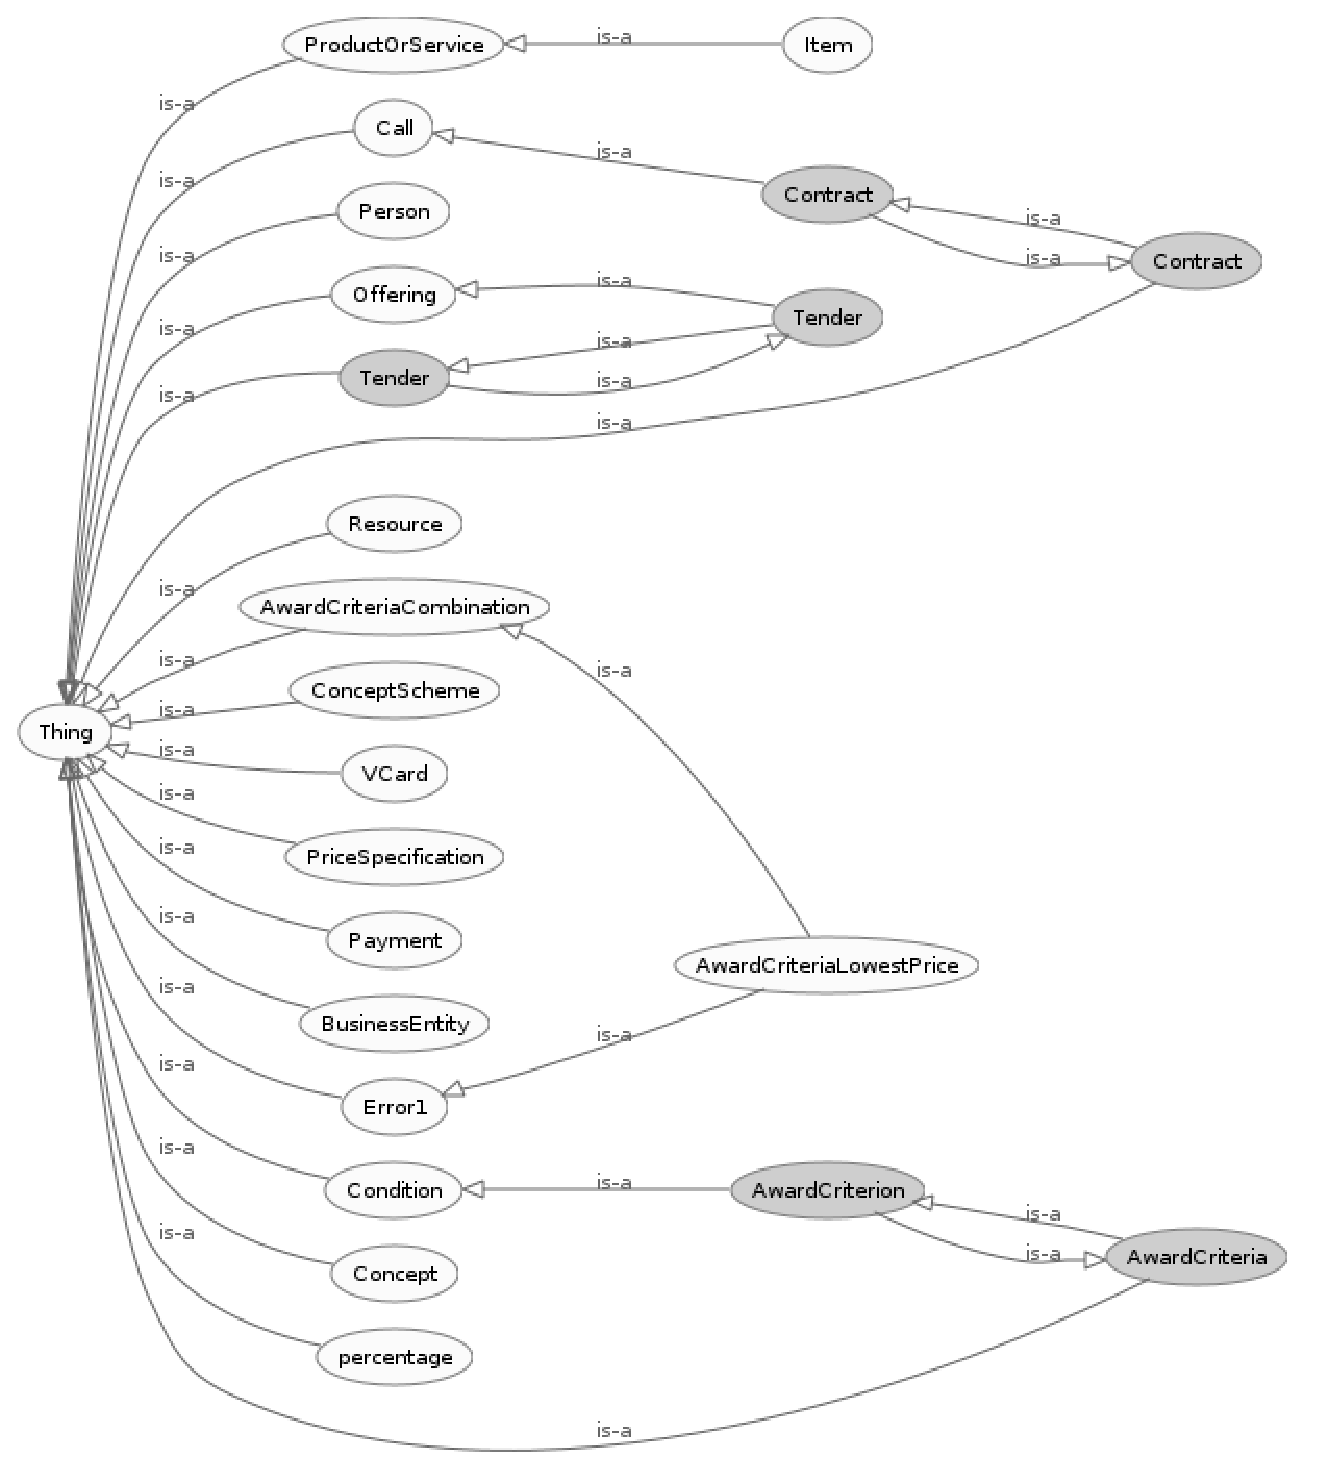
\includegraphics[width=14cm]{images/phd/public-contracts-ontology}
  \caption{\textit{Public Contracts Ontology from Czech Republic.}}
 \label{fig:public-contracts-ontology}
\end{figure}


\subsubsection{Clasificaciones Estándar de Productos}\label{semantica:pscs}
Las clasificaciones de productos, son instrumentos claves de estandarización~\cite{Leukel-standard} que nacen con el fin de
conseguir una clasificación común de productos y servicios. En general, son variadas~\cite{Leukel-ecatalog2005}
y obedecen a intereses particulares dependiendo del sector como e@Class o RossetaNET,
o bien de carácter global como \gls{UNSPSC} u otras destinadas a un dominio particular como el \gls{CPV} en la Administración Pública, ver Sección~\ref{sect:pscs}. Las diferencias
estriban en su alcance y cobertura sectorial, pero también en el grado de especificidad o nivel
de profundidad que existe para describir los productos o servicios.

Como señala Hepp\cite{HeppTrueComplexity,HeppEclass,HeppMethodology} todos estos
estándares reflejan una combinación de componentes variables, que pueden ser
utilizados para la construcción de una ontología derivada a partir de la clasificación.
Sin embargo, se puede identificar una estructura común subyacente a todas ellas y
que es fundamental señalar para proporcionar un modelo de datos semántico universal para este tipo de clasificaciones, consistente 
en que todas estas clasificaciones se ordenan jerárquicamente. 

\begin{description}
 \item [Categorías de productos.] Las clasificaciones se dividen en categorías o
clases de productos, agrupando los distintos elementos del catálogo.
\begin{itemize}
 \item Las categorías de la clasificación se organizan jerárquicamente.
 \item Cada elemento de la clasificación pertenece a una categoría de
productos.
 \item Cada elemento de la clasificación pertenece sólo una categoría de
productos, es decir, las categorías son disjuntas.
\end{itemize}

\item  [Estructura taxonómica.] Además de la división en niveles de jerarquía
de los elementos de la clasificación, su objetivo es organizar y agrupar los productos en
sectores verticales mediante algún tipo de criterio establecido por la comunidad
que desarrolla el estándar. 
 
\end{description}

Estas son características genéricas de las clasificaciones de productos. Sin
embargo, otras clasificaciones más sofisticadas incluyen un diccionario de propiedades
estándar que se puede utilizar para describir productos con más detalle.
Normalmente, estos diccionarios de propiedades también incluyen los tipos de
datos que pueden ser valor de las mismas, así como su referencia con respecto a estándares internacionales para establecer las unidades de medida, este es el caso
de la clasificación de productos de e@Class. En otras ocasiones, se construyen
clasificaciones multiling\"{u}es para la expresión de los descriptores de cada
elemento. 

La irrupción de la tecnología semántica y, sobre todo, la aparición de
lenguajes web para la representación de conocimiento y gestión de metadatos, ha
propiciado un creciente interés en el uso de las clasificaciones estándar de productos para mejorar tanto el
intercambio de información, como su capacidad para estructurar información. La construcción de ontologías de productos 
con alto nivel de detalle implican un coste que es muy difícil de asumir en muchos casos. 
Los autores~\cite{Yu:2009:CSI:1693684.1693743,FenselOmel2001,FenselDing2001} comparten la opinión de Corcho~\cite{CorchoECommerce} 
de que una ontología de productos sería muy útil para la organización conceptual del mercado, se entiende que estas ontologías tienen
más carácter privado, para la organización de la producción, los departamentos
de ventas y comerciales y, en general, para cualquier área de una empresa o
institución que deba tratar con la gestión de productos.

El desafío básico más importante que hay que afrontar cuando se deriva una
ontología de una clasificación de productos, se refiere a cómo interpretar la semántica original de la taxonomía.
No existe una definición formal de las relaciones taxonómicas que construyen
cada categoría de la clasificación y es tentador utilizar la propiedad de un
vocabulario de ontologías, como \textit{rdfs:subClassOf}, para intentar
representar estas relaciones semánticas, sin embargo, esta suposición es errónea. Como señala~\cite{HeppMethodology}, esta relación de jerarquía entre los elementos no se puede considerar
equivalente a una relación de subclase o de herencia. En primer
lugar, tomando el siguiente ejemplo: el elemento ``Partes y accesorios de
bicicleta'' del \gls{CPV} 2008 (34432000-4) tiene como antecesor a ``Bicicletas''
(34440000-0), donde la relación semántica entre los dos elementos no es
herencia, es decir, no se puede expresar que una \textbf{parte de una bicicleta}
sea una \textbf{bicicleta}. Para ser más precisos, debería modelarse como una relación de
composición o agregación. En este sentido, ocurre igual con la relación
taxonómica entre ``Tubos de resina Epoxi''(19522110-5) y ``Resina Epoxi''
(19522100-2), en el que es difícil justificar de nuevo una relación de herencia
clásica entre el primero y el segundo elemento del CPV, ya que en ningún caso
se puede considerar que el continente y el contenido de un objeto complejo tenga
el mismo estatus en una ontología de dominio, es decir, que un \textbf{tubo} no
es un tipo de \textbf{resina}.

Pero no sólo es complicado interpretar correctamente las relaciones semánticas
que codifica la taxonomía de una clasificación de productos, desde el punto de vista de las ontologías
como modelos de conocimiento de dominio, muchos elementos de una clasificación de productos son
difícilmente interpretables como conceptos de dominio, en este sentido, un elemento como ``Barras, varillas, perfiles y alambre de
estaño'' (27623100-9) del CPV 2003, que parece más una colección
artificial de productos que una clase estructural, en la que sus instancias
comparten algún tipo de propiedad común, estrictamente para
interpretar correctamente el elemento ``Barras, varillas, perfiles y alambre de
estaño'' como una clase, debería definirse como la unión de varias clases:
por ejemplo, ``Barras'', Varillas`` o ''Alambre de estaño``.

La problemática que presenta el modelado semántico de las clasificaciones de productos
conlleva dificultades intrínsecas que no se encuentran en otros dominios. En este
sentido han surgido vocabularios como \textit{GoodRelations} y \textit{ProductOntology}, que facilitan
estas tareas de modelado y reutilización de descripciones de productos. \textit{GoodRelations}
es un vocabulario estándar (esquema, diccionario u ontología) para productos y datos empresariales 
que pueden ser introducidos en páginas web, ver Figura~\ref{fig:rdf-gr} de las tripletas
extraídas utilizando el servicio \textit{Any23}, tanto estáticas como dinámicas, para permitir de esta forma el procesamiento automático por las máquinas. La principal ganancia
reside en el aumento de la visibilidad, por motores de búsqueda etc., de los productos y servicios 
etiquetados de esta manera, actualmente algunas de las empresas que utilizan este vocabulario
son: Google, Yahoo, Best Buy, O'Reilly, Volkswagen UK, Renault UK, etc., en general para etiquetar
sus productos y para que la información pueda ser procesada automáticamente.

\begin{figure}[!htbp]
\centering
  \begin{lstlisting} 
<http://www.renault.co.uk/ownerservices/shop/item/renaulttoys/pedalcar/eco2pedalcar/default.aspx> 
  dcterms:title "ECO2 Pedal Car - Renault Shop - Owner Services - Renault UK" .


<http://www.renault.co.uk/ownerservices/shop/item/renaulttoys/pedalcar/eco2pedalcar/default.aspx#offering> a 
  <http://purl.org/goodrelations/v1#Offering> .

<http://www.renault.co.uk/ownerservices/shop/item/renaulttoys/pedalcar/eco2pedalcar/default.aspx#offering> 
  gr:eligibleRegions  "GB"^^<http://www.w3.org/2001/XMLSchema#string> .


<http://www.renault.co.uk/ownerservices/shop/item/renaulttoys/pedalcar/eco2pedalcar/default.aspx#offering> 
	foaf:page <http://www.renault.co.uk/ownerservices/shop/item/RenaultToys/PedalCar/ECO2PedalCar/default.aspx> ;
	gr:availableDeliveryMethods <http://www.renault.co.uk/ownerservices/shop/deliverydetails.aspx#delivery> ;
	gr:hasPriceSpecification <http://www.renault.co.uk/ownerservices/shop/deliverydetails.aspx#deliverycharges> ;
	gr:name "ECO2 Pedal Car" ;
	gr:hasPriceSpecification _:node16kpidu7qx455 .

_:node16kpidu7qx455 a gr:UnitPriceSpecification ;
	gr:hasCurrency "GBP"^^<http://www.w3.org/2001/XMLSchema#string> ;
	gr:hasCurrencyValue "260"^^<http://www.w3.org/2001/XMLSchema#float> ;
	gr:valueAddedTaxIncluded "true"^^<http://www.w3.org/2001/XMLSchema#boolean> ;
	gr:validThrough "2012-02-03T17:22:43Z"^^<http://www.w3.org/2001/XMLSchema#datetime> ;
	gr:hasUnitOfMeasurement "C62"^^<http://www.w3.org/2001/XMLSchema#string> .

<http://www.renault.co.uk/ownerservices/shop/item/renaulttoys/pedalcar/eco2pedalcar/default.aspx#offering> 
      gr:hasBusinessFunction gr:Sell ;
	gr:hasInventoryLevel _:node16kpidu7qx456 .

_:node16kpidu7qx456 a gr:QuantitativeValue ;
	gr:hasMinValue "1"^^<http://www.w3.org/2001/XMLSchema#float> .

<http://www.renault.co.uk/ownerservices/shop/item/renaulttoys/pedalcar/eco2pedalcar/default.aspx#product> a gr:SomeItems ;
	gr:category "Pedal Car" ;
	gr:name "ECO2 Pedal Car" ;
	gr:description "Dimensions: 114 x 69 x 62cm. Weight: 10kg. Age 3 to 7 years." ;	
	foaf:page <http://www.renault.co.uk/ownerservices/shop/item/RenaultToys/PedalCar/ECO2PedalCar/default.aspx> .
  \end{lstlisting}
\caption{Ejemplo de tripletas de RDF en N3 extraídas de un producto de Renault utilizando \textit{GoodRelations}.}
\label{fig:rdf-gr}
\end{figure}  

Por otra parte, \textit{ProductOntology} se utiliza para enlazar cualquier producto con una descripción
que está disponible en la Wikipedia, de esta manera las instancias de la ontología obtienen una
definición dinámica que se puede reutilizar en cualquier contexto. Finalmente, cabe destacar
la iniciativa \textit{schema.org} desarrollada por los grandes proveedores de servicios de búsqueda, 
cuyo objetivo es encajar descripciones en las propias páginas web para que el descubrimiento
de la información por parte de los \textit{crawlers} sea más sencillo.

En cuanto a los escenarios o casos de uso en los que las catálogos de clasificaciones de productos
han sido utilizados son variados, pero podrían destacarse los siguientes: en servicios web semánticos
para el proceso de descubrimiento, para el intercambio y actualización automática de catálogos
de productos entre distintas aplicaciones, para el etiquetado de recursos mediante vocabularios
controlados, etc. Como conclusión, se puede observar que las clasificaciones de productos y servicios son sumamente interesantes
para la mejora de la interoperabilidad e integración de las aplicaciones, que ha sido ampliamente impulsada por la irrupción de la corriente 
de la Web Semántica y los datos enlazados.


%FIXME
% Nuestra postura es radicalmente distinta. Desde nuestro punto de vista, las PSCs
% fueron construidas para solucionar problemas de comunicación, proporcionar una
% forma de organizar tipos de productos y agruparlos acuerdo a unos conceptos y
% definiciones que funcionasen \textit{de facto} como un estándar en determinados
% entornos de actividad comercial e industrial. Las PSCs no fueron diseñadas como
% modelos conceptuales de dominio, en el sentido actual que tiene el término
% ``ontología'', sino como una forma de estructurar la terminología y la forma de
% nombrar a los productos. De ahí, que interpretemos las PSCs como simples
% esquemas conceptuales en el que la relación taxonómica que jerarquiza los
% distintos elementos de cada $T_{psc}$ no se interpreta como una relación de
% herencia o subtipo, sino como una relación de mayor o menor especificidad de los
% elementos. Resumiendo, consideramos las PSCs como simples vocabularios
% controlados y utilizaremos una ontología RDF/OWL, SKOS Core, como modelo de
% datos común.


\subsubsection{Información sobre Organizaciones}\label{sect:orgs}
En el caso de las organizaciones la tarea de búsqueda de propuestas relacionadas
con semántica se complica debido a que existen numerosas ontologías que tienen
definido el concepto de ``Organización''. Por ejemplo \gls{FOAF} hace uso de esta entidad
para referirse a la compañía a la que pertenece una persona, \textit{Inference Web} que 
está estrechamente relacionada con procesos de inferencia en la web, en el ámbito de \textit{trust} y \textit{provenance}~\cite{prov-group}, 
utiliza las organizaciones para establecer la relación de confianza que existe entre las diferentes entidades. En todos los casos
la representación y cobertura del concepto ``Organización'' es mínimo y adaptado
para el caso particular.

Según la evaluación realizada por Dave Reynolds (Epimorphics Ltd) en un informe web~\cite{org-ontology}, convertido 
en los últimos tiempos en borrador~\cite{dave-w3c} del \gls{W3C}, se han desarrollado muchos enfoques los cuales estaban dirigidos por distintos objetivos, algunos centrados 
en la noción de organización como ente superior, así aparece en \textit{upper-ontologies} como Proton, Sumo o SmartWeb. Estos modelos están construidos con múltiples objetivos, 
por lo que en principio no se adaptan fácilmente a la estructura de modelos pequeños y reutilizables 
para la descripción de las organizaciones, aunque evidentemente deben ser revisados. Por otra parte,
si se utilizan los motores de búsqueda para obtener los trabajos relacionados con las organizaciones, Swoogle obtiene 
alrededor de $3.900$ resultados, Falcons $15,881$ del concepto ``Organization''
estando presente en 15 vocabularios diferentes y Google ofrece: 1) la ``Organization Ontology 1.0'' desarrollada
en SHOE la cual proporciona una idea de la jerarquía básica de una organización, industrias y roles posibles de los empleados;
2) una ``Organization Ontology for Enterprise Modelling'', más orientada a entornos de cadenas
de suministros y 3) ``Enterprise Ontology'', que es una ontología para representar la actividad de negocio
de las empresas en Ontolingua. También \textit{Jeni Tennison}, a través de su blog, ha apuntado a la ontología
desarrollada por TSO para ``London Gazette \gls{RDFa} markup'', en la cual se incluyen los conceptos de ``Gazzete Organization''
y ``Gazette Person''. 

En general, se pueden sintetizar que los enfoques llevados a cabo en AKT Portal Ontology, Proton,
\textit{GoodRelations}, \gls{FOAF}, \gls{SIOC}, \textit{Enterprise Modelling Ontology}, \textit{Enterprise Ontology}, \textit{Gazzete}, \textit{Provenance Vocabulary Ontology}
y otros orientados al ambiente académico como ECS (Universidad de Southampton) o ``Academic Institution Internal Structure Ontology'' (\gls{AIISO}), 
deben ser tenidos en cuenta para obtener una enseñanza común y un vocabulario que pueda describir de forma genérica
y extensible la casuística que surge para modelar la información empresarial. En conclusión, existe 
un amplio conjunto de vocabularios destinados a describir entidades similares pero con distintos objetivos
y que se han reutilizado en la ontología de Organizaciones, ver Figura~\ref{fig:org-ontology}, desarrollada por Dave Reynolds. Este trabajo
es un excelente punto de partida para el modelado de organizaciones en la \wode ya que ha condensado el conocimiento
previo.

\begin{figure}[h]
 \centering
    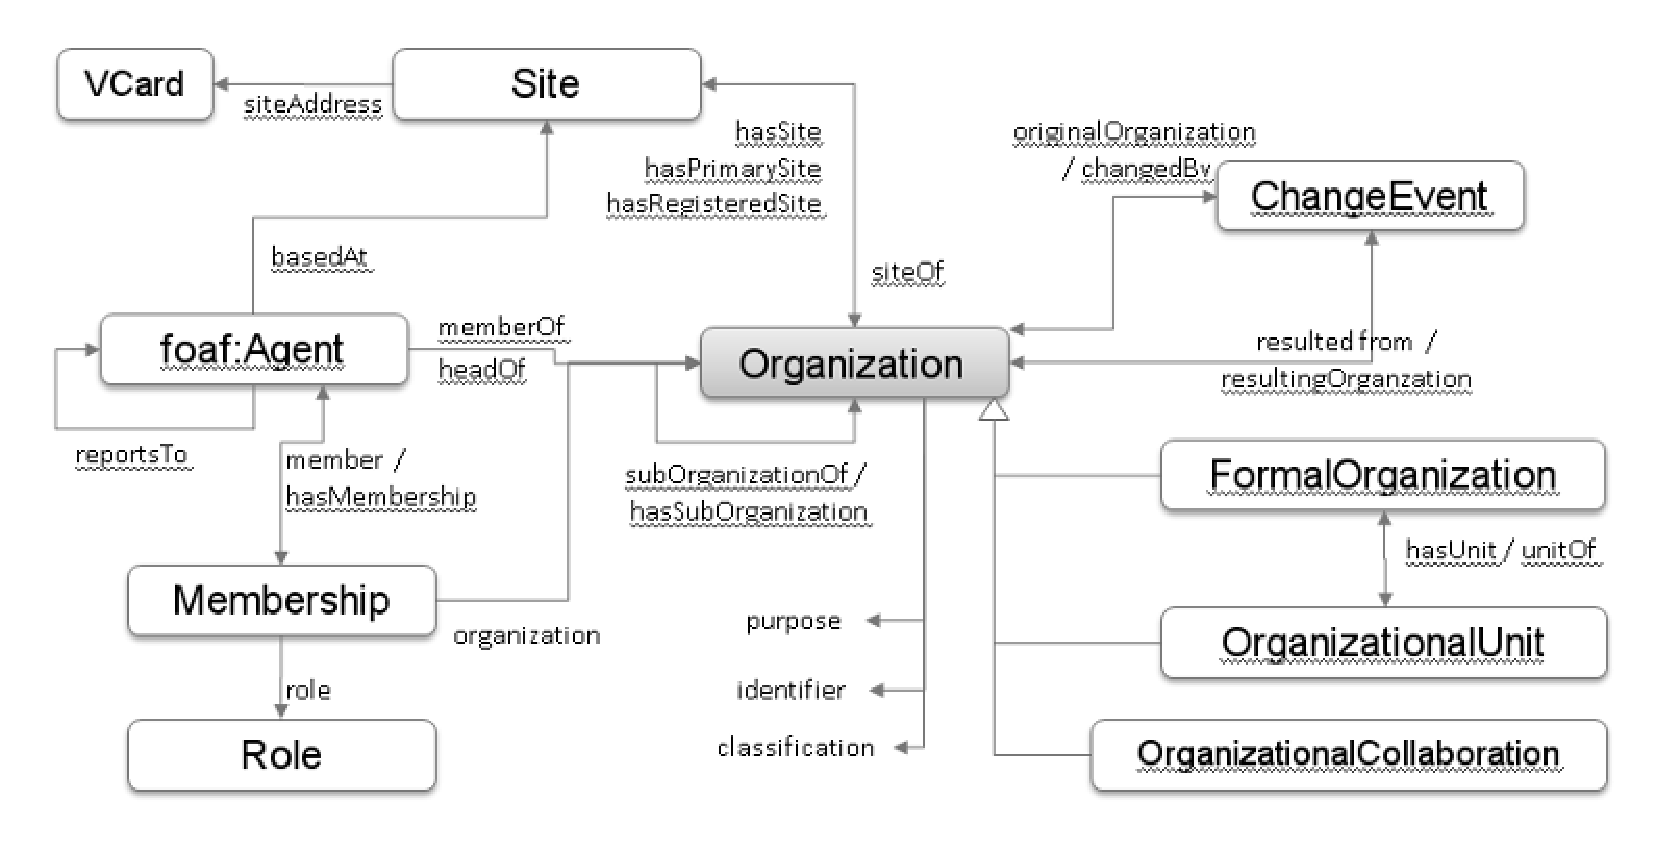
\includegraphics[width=14cm]{images/phd/org}
  \caption{\textit{Organizations Ontology. Overview.}}
 \label{fig:org-ontology}
\end{figure}

Desde otro punto de vista no tan centrado en la corriente de Web Semántica y ontologías, hay que referenciar 
la propuesta de datos abiertos realizada por \textit{OpenCorporates} a través ``\textit{The Open Database Of The Corporate World}'', han utilizado
técnicas de \textit{screen scrapping} y \textit{crawling} para extraer información de más de $12$ millones de compañías. Esta
información, ver Figura~\ref{figure:open-org}, tiene un alto valor para reutilizar y trazar la actividad de una empresa ya que disponen en la mayoría
de los casos del identificador de la empresa. La información de esta base de datos sigue un enfoque mixto entre \opendata y \linkeddata, 
pero el gran problema reside en la ausencia de un modelo formal para la descripción de los datos, es por ello que disponer de un modelo formal 
que integre esta información es clave para la posible reutilización de la información y explotación de la misma de una forma estándar.

\begin{figure}[!h]
\begin{center}
\begin{lstlisting}[language=SPARQL]
    <http://opencorporates.com/companies/nl/37136346.rdf?id=5828504>    
      a <http://purl.org/dc/dcmitype/Text>,
                foaf:Document;
         dct:format "application/rdf+xml";
         dct:isFormatOf 
	  <http://opencorporates.com/companies/nl/37136346?id=5828504>;
         dct:title "Linked Data in RDF format for Benuma";
         foaf:primaryTopic 
	  <http://opencorporates.com/id/companies/nl/37136346> .
	  ...
        <http://opencorporates.com/id/companies/nl/37136346>     
	a <http://s.opencalais.com/1/type/er/Company>;
         :label "Benuma" 
\end{lstlisting}
\caption{Información (parcial) sobre una Organización de ``Open Corporates'' en N3.}
\label{figure:open-org}
\end{center}
\end{figure}

\cleardoublepage
\subsubsection{Proyectos de Investigación}
Los proyectos de investigación de los principales programas competitivos
también se han visto involucrados en el despliegue de sistemas de contratación
pública electrónica utilizando semántica y datos enlazados. Entre ellos
se pueden destacar los siguientes:
\begin{description}
 \item [\textit{LOTED Project}~\cite{loted-project}] \textit{Linked Open Tenders Electronic Daily} realizado
por el grupo KMI de la \textit{Open University} del Reino Unido permite la consulta en \gls{SPARQL} de anuncios de licitación
publicados a través de los \gls{RSS} de \gls{TED}. Se trata del tradicional enfoque de \textit{Rdfizar}, información
ya publicada y hacerla disponible a través de un \textit{endpoint} de SPARQL. Sin duda se trata
de una importante iniciativa tanto por su carácter innovador, como por tratarse de la primera apuesta
real de utilización de semántica en los anuncios de licitación, sin embargo, tan sólo llega a los anuncios
de licitación publicados en TED y también parece que el demostrador oficial ha dejado de ser 
mantenido por los autores. No obstante, es necesario considerar esta propuesta para aprovechar
el efecto experiencia de la misma.
 \item [\textit{LOD2 Project}~\cite{lod2-project}.] Este proyecto europeo al que se ha referenciado en la
Sección~\ref{lod2-project} por su esfuerzo en la iniciativa \linkeddata desde un punto de vista genérico, también ha seleccionado la contratación pública electrónica como un caso de uso estratégico, es por ello
que han aumentado los paquetes de trabajo para incluir el esfuerzo de la \textit{Charles University} de la República Checa y su investigación sobre la aplicación de \linkeddata y semántica en el campo
del \eproc. Esto se ha manifestado en la constitución del paquete de trabajo \textit{WP9A – LOD2 for a Distributed Marketplace for Public Sector Contracts}.
La importancia del seguimiento de este proyecto reside tanto en las personas como en las instituciones implicadas, ya que generan 
una gran cantidad de tecnología y \textit{know-how} especialmente relevante para el estudio objeto de este documento y para las iniciativas
de \linkeddata y \opendata en general.
 \item [\textit{LATC Project}~\cite{latc-project}.] \textit{Linked open data around-the-clock} es un proyecto europeo,
una \textit{Specific Support Action} en el contexto del 7º Programa Marco-ICT formado por más de 58 instituciones
en los que se realizan y coordinan proyectos, personas. etc. El objetivo de este proyecto es gestionar la información
y datos generados a través de distintas fuentes proveyendo la infraestructura y documentación necesaria para
desplegar arquitecturas que den soporte a los datos enlazados. Prueba de su ingente capacidad es la cobertura y 
asesoramiento a proyectos y a investigadores de Europa (74\%) y de Estados Unidos (25\%). El consorcio
está formado por instituciones y empresas tan relevantes en este campo como: \textit{Digital Enterprise Research Institute} (DERI), \textit{NUI Galway}, Irlanda;
\textit{Vrije Universiteit Amsterdam} (VUA), Países Bajos; \textit{Freie Universit\"{a}t Berlin} (FUB), Alemania; \textit{Institute for Applied Informatics} e.V. (InfAI), Alemania y
\textit{Talis Information Ltd.}, Reino Unido.

\item [\textit{PlanetData Project}~\cite{planet-data-project}.] Se trata de una Red de Excelencia en el 
ámbito europeo (FP7-257641) con un presupuesto total de $3.72$ millones de euros y en la que participan los principales 
organismos de investigación con el objetivo de sumar los esfuerzos de la comunidad de investigadores para ofrecer 
a las organizaciones interesadas en la iniciativa de \linkeddata soporte con la publicación de sus datos. Evidentemente 
cuentan con un estrecho lazo con los proyectos anteriores y su actividad cubre las cuestiones relacionadas con datos enlazados 
en diferentes ámbitos: \textit{data streams, (micro) blog posts, digital archives, eScience resources, public sector data sets, and the Linked Open Data Cloud}.

\item [\textit{WebDataCommons.org}~\cite{web-data-commons-project}.] Es una iniciativa conjunta realizada por el grupo 
de investigación \textit{Web-based Systems Group} en la \textit{Freie Universit\"{a}t} de Berlín y el 
\textit{Institute AIFB} perteneciente al \textit{Karlsruhe Institute of Technology}, en el cual se han extraído 
y generado tripletas \gls{RDF} de más de $65$ millones de sitios web, contando un número de 
\textit{$3.2$ billion RDF quads} a fecha de febrero del año 2012, cubriendo información sobre productos, 
personas, organizaciones, lugares, eventos y recetas de cocina entre otros. Para la realización de este 
experimento se han utilizando técnicas de extracción de información de \gls{HTML} que utilizan microformatos, RDFa, etc. 
Toda esta información y datos está disponible para su descarga y uso por terceros en RDF. La importancia de este proyecto 
reside tanto en las personas y organizaciones implicadas como en la magnitud de los datos que han conseguido extraer.

\item [Otros proyectos.] Estas iniciativas trabajan con tecnología semántica y de datos enlazados en diferentes contextos suministrando servicios
a instituciones públicas o bien realizando investigación e innovación. Entre otros, se pueden citar: \gls{FP7} project SEALS (\textit{Semantic Evaluation at Large Scale}), FP7 project SpitFIRE (\textit{Semantic-Service Provisioning for the Internet of Things using Future Internet Research 
by Experimentation}), French DataLift project y Semic.EU.
\end{description}

Igualmente a nivel nacional se han impulsado diferentes iniciativas
y proyectos, como los de la República Checa y ``10ders Information Services'', que intentan elevar el significado de la información
de los anuncios de licitación utilizando tecnologías semánticas. También hay que considerar que la reutilización
de vocabularios ya establecidos e impulsados por las distintas Administración Públicas, por ejemplo la iniciativa Joinup~\cite{joinup-europe} de la Unión Europea, 
es de suma relevancia para proporcionar información utilizando datos enlazados, en este sentido todas las iniciativas y proyectos reseñados en las secciones anteriores ayudan a 
disponer de los \textit{building blocks} necesarios para afrontar la aplicación de semántica a los procesos de contratación pública electrónica.

% 10-15


\printindex
\printglossaries


% Bibliografía
\insertbibliography
\end{document}
